\documentclass[12pt, draftclsnofoot, onecolumn]{IEEEtran}
\usepackage{amsmath,amsfonts}
\usepackage{algorithmic}
\usepackage{algorithm}
\usepackage{array}
\usepackage[caption=false,font=normalsize,labelfont=sf,textfont=sf]{subfig}
\usepackage{textcomp}
\usepackage{stfloats}
\usepackage{url}
\usepackage{verbatim}
\usepackage{graphicx}
\usepackage{cite}
\usepackage{xcolor}
\usepackage{lineno}
\linenumbers

\begin{document}
\title{Localization of Subsea CO$_2$ Leak Source Using Bio-inspired Robotic Fish}

\author{Muhammad Umar Masood$^{1}$, Qiang Zhu$^{1}$ and Zheng Chen$^{2}$% <-this % stops a space
\thanks{*This research is supported by the Center of Carbon Management for Energy at UH Energy}% <-this % stops a space
\thanks{$^{1}$Muhammad Umar Masood, Qiang Zhu and Zheng Chen are with the Department of Mechanical and Aerospace Engineering, University of Houston, Texas, United States.
{\tt\small mmasood8@uh.edu, zhu21@uh.edu, zchen43@uh.edu}}%
}
\maketitle

\begin{abstract}
This paper introduces the design and experimental evaluation of AquaNavigator, a robotic fish capable of full three-dimensional maneuvering. The platform can carry one or more sensors for environmental safety applications and can measure underwater parameters such as dissolved carbon dioxide. Although direct depth localization using Global Positioning Systems (GPS) is not feasible underwater, this work proposes a method in which data are collected below the surface and then associated with the robot’s next available surface position. For testing and validation, experiments are conducted in an indoor water tank, where an overhead camera is employed to emulate the localization system. A CO$_2$ pipeline leak is created at the bottom of the tank, and the trials demonstrate that the robotic fish can identify the region of CO$_2$ leakage. Additional data analysis methods are then applied to refine the estimate of the leak’s source location. Experimental results indicate that the leakage origin can be determined with an error of 0.69~m.
\end{abstract}
\begin{IEEEkeywords}
Bio-inspired robotic fish, CO$_2$ monitoring, underwater robotics, robotic fish design
\end{IEEEkeywords}

\section{INTRODUCTION}
Due to the extensive use of fossil fuels, atmospheric carbon dioxide (CO$_2$) concentrations have been rising rapidly, driving global warming and climate change \cite{Filonchyk2024,Kabir2023}. To address these impacts, carbon capture and storage (CCS) technologies have been introduced to remove CO$_2$ emissions from power plants and industrial operations and permanently store them underground or at offshore sequestration sites \cite{Herzog2001,Yadav2022,Osman2021}. With emerging policies and regulations in the United States and other nations, a reduced carbon footprint now provides companies with a competitive edge. Therefore, it is crucial for regulatory authorities to verify that the captured carbon is securely contained at offshore sequestration locations, rather than escaping and mixing into low-pressure aquatic environments.

Leaked CO$_2$ from underwater pipelines and sequestration sites can have more severe impacts on the environment and marine ecosystems than the CO$_2$ that remains in the atmosphere and is not captured \cite{Zheng2021,Mortezaei2021}. Consequently, once CO$_2$ is captured, its safe transport and storage become critically important from both environmental and economic standpoints. In current practice, CO$_2$ is conveyed in a supercritical state through subsea pipelines to storage sites. The literature shows that the presence of impurities in CO$_2$, together with its supercritical state, can induce phase transitions that create a decompression plateau, which in turn can drive long-distance crack propagation along the pipeline and lead to serious failures \cite{Aursand2016,CoshamAtkinsBoreas2009}. In addition, these pipelines are susceptible to leakage caused by corrosion, material flaws, and external mechanical damage. Escaped CO$_2$ can dissolve into seawater and form carbonic acid, lowering the pH and posing a threat to marine organisms \cite{queiros2014potential,Pham2016}. Hence, continuous monitoring of underwater pipelines for potential CO$_2$ leakage and the implementation of appropriate preventive measures are vital to avoiding environmental harm.

Extensive research has been carried out on inspecting subsea pipeline leaks using Autonomous Underwater Vehicles (AUVs) and Remotely Operated Vehicles (ROVs). Zhang et al. \cite{Zhang2021} introduced an AUV capable of identifying gas leaks in subsea pipelines by visually detecting gaseous bubbles in water. Although this system is not tailored specifically to CO$_2$ leak detection, it nonetheless represents a significant step toward underwater pipeline leak monitoring. Qasem et al. \cite{Qasem2019} proposed a multi-sensor ROV designed for oil spill surveillance. In addition, some studies have explored bio-inspired robotic fish for leakage detection. For instance, Hu et al. \cite{Hu2022} developed a robotic fish to identify bubble leaks in underwater pipelines, employing advanced Artificial Intelligence (AI) algorithms to detect bubbles via an on-board camera. However, all these systems are technologically sophisticated, costly, and still do not offer a dependable solution for detecting CO$_2$ leaks in particular.

Monitoring, preventive maintenance, and inspection of offshore assets and the surrounding ecosystem have been standard practices in the oil and gas sector for decades \cite{Shukla2016,Mcleod2012,Patel2024}. These tasks are typically carried out using Remotely Operated Vehicles (ROVs) and Autonomous Underwater Vehicles (AUVs), which demand specialized operator teams and entail high operational costs. Such expenses are generally acceptable when dealing with the upkeep and inspection of high-value infrastructure. However, conventional ROVs are not well integrated with the marine ecosystem and may disturb marine life \cite{Polverino2013,Marras2012}. In contrast, bio-inspired robotic fish offer a potentially cost-effective alternative that is better aligned with the natural ocean environment and minimizes ecological disturbance.

In this work, a solution to the aforementioned problem is introduced through the development of a novel bio-inspired robotic fish, AquaNavigator, designed for monitoring underwater CO$_2$ pipelines for potential leaks. The robot emulates the swimming patterns of real fish, enabling it to move through the water with minimal disruption to marine life. It is outfitted with a CO$_2$ sensor capable of detecting CO$_2$ concentrations in the water, logging the collected data, and associating it with the nearest likely surfacing location. AquaNavigator can be deployed in subsea environments to inspect CO$_2$ pipelines for possible leakages and deliver real-time information to operators. In this study, an indoor water tank is employed to emulate the operating conditions, with a camera mounted above it to replicate the localization system. A CO$_2$ pipeline leak is created at the bottom of the tank, and the experiments confirm that the robotic fish can successfully locate the CO$_2$ leakage area. The experimental findings validate the effectiveness of the proposed method for monitoring underwater CO$_2$ pipelines and detecting potential leaks.



\section{DESIGN AND DYNAMICS OF AQUANAVIGATOR}{\label {sec:design}}
AquaNavigator is a novel bio-inspired robotic fish designed to mimic the swimming behavior of real fish. The robotic fish is designed to be compact, lightweight, and easy to maneuver in the water. The design of AquaNavigator is inspired by the morphology and swimming behavior of real fish, which allows it to navigate through the water with minimal disturbance to the marine life. The undulatory motion can be described by the traveling wave equation as introduced by Lighthill \cite{Lighthill1969}:
\begin{equation}
y(x,t) = \big(c_1 x + c_2 x^2\big) \sin(kx + \omega t)
\end{equation}
where $y$ is the lateral displacement of the fish body at position $x$ along the body length and time $t$, $c_1$ and $c_2$ are coefficients that define the amplitude envelope of the wave, $k$ is the wave number, and $\omega$ is the angular frequency of the wave. This equation can be discretized, and thus for the case of a robotic fish, it needs at least two joints to mimic the undulatory motion, and it becomes:
\begin{equation}
    y_i(x_i,t) = \big(c_{1i} x_i + c_{2i} x_i^2\big) \sin(k_i x_i + \omega t) \forall i=1,2
\end{equation}
To acheive this motion, the robotic fish tail uses a double slider-crank mechanism \cite{Masood2025} which uses one actuator to generate this wave motion with a fixed phase difference between the two joints, denoted as $\phi_1$. The detailed modeling and design of the robotic fish is presented in \cite{Masood2025}, which is an improved version of its squeal \cite{Zuo2021}. The depth control mechanism comes from \cite{Masood2023}. \\
AquaNavigator consists of a water tight enclosure for the circuitry, battery, buoyancy control mechanism and other prone-to-water components, a double slider-crank mechanism for tail fin actuation powered by a geared DC motor, and high-torque servo motor for the tail bias angle. Other than the water tight enclosure, all the components are individually water-proofed with marine compatible resin epoxy coatings. All the parts are 3D printed with SLA based resin printer, which provides high strength and durability. It is equipped with a three cell (3s) lithium-polymer (Li-Po) 2200 mAh battery pack for power and an ESP32-C3 microcontroller from Espressif Systems for control and communication. The robotic fish is also equipped with a Near Infrared (NIR) CO$_2$ sensor for detecting the diffused CO$_2$ levels in water. The detailed specifications of the robotic fish are presented in Table \ref{tab:specs} and the annotated CAD model of the robotic fish is shown in Fig. \ref{fig:cad_model}. The fabricated real robotic fish is shown in Fig. \ref{fig:real_robotic_fish}.
\begin{figure}[ht]
    \centering
    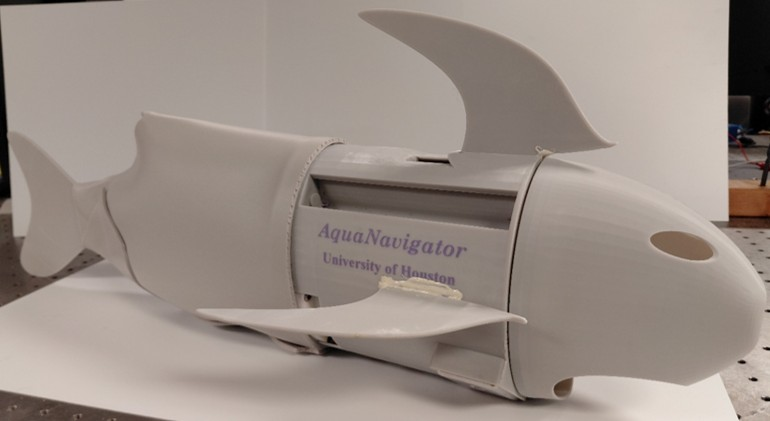
\includegraphics[width=0.6\textwidth]{Fig/Real-Fish.jpg} 
    \caption{Fabricated AquaNavigator robotic fish.}
    \label{fig:real_robotic_fish}
\end{figure}
\begin{table}
\caption{Specifications of AquaNavigator Robotic Fish}
\label{tab:specs}
\centering
\begin{tabular}{|l|l|l|}
\hline
\textbf{Parameter}               & \textbf{Value}            & \textbf{Unit}        \\ \hline
Speed                         & 0.2                 & m/s                  \\ \hline
Speed                         & 0.3                 & BL/s                  \\ \hline
Length                        & 0.67                & m                    \\ \hline
Swim Style                    & Carangiform     & -                    \\ \hline
Weight                        & 2.5                 & kg                   \\ \hline
Depth Rating                  & IP67                  & -                  \\ \hline
Depth Control Range          & 17.88              & m                    \\ \hline
Battery Life                  & 40                  & min                  \\ \hline
Operation Distance        & 480                  & m                    \\ \hline
On-board Sensors & \begin{tabular}{@{}l@{}}NDIR CO$_2$ sensor\\IMU\\Depth\\Camera\end{tabular} & - \\ \hline
\end{tabular}
\end{table}
\begin{figure}[ht]
    \centering
    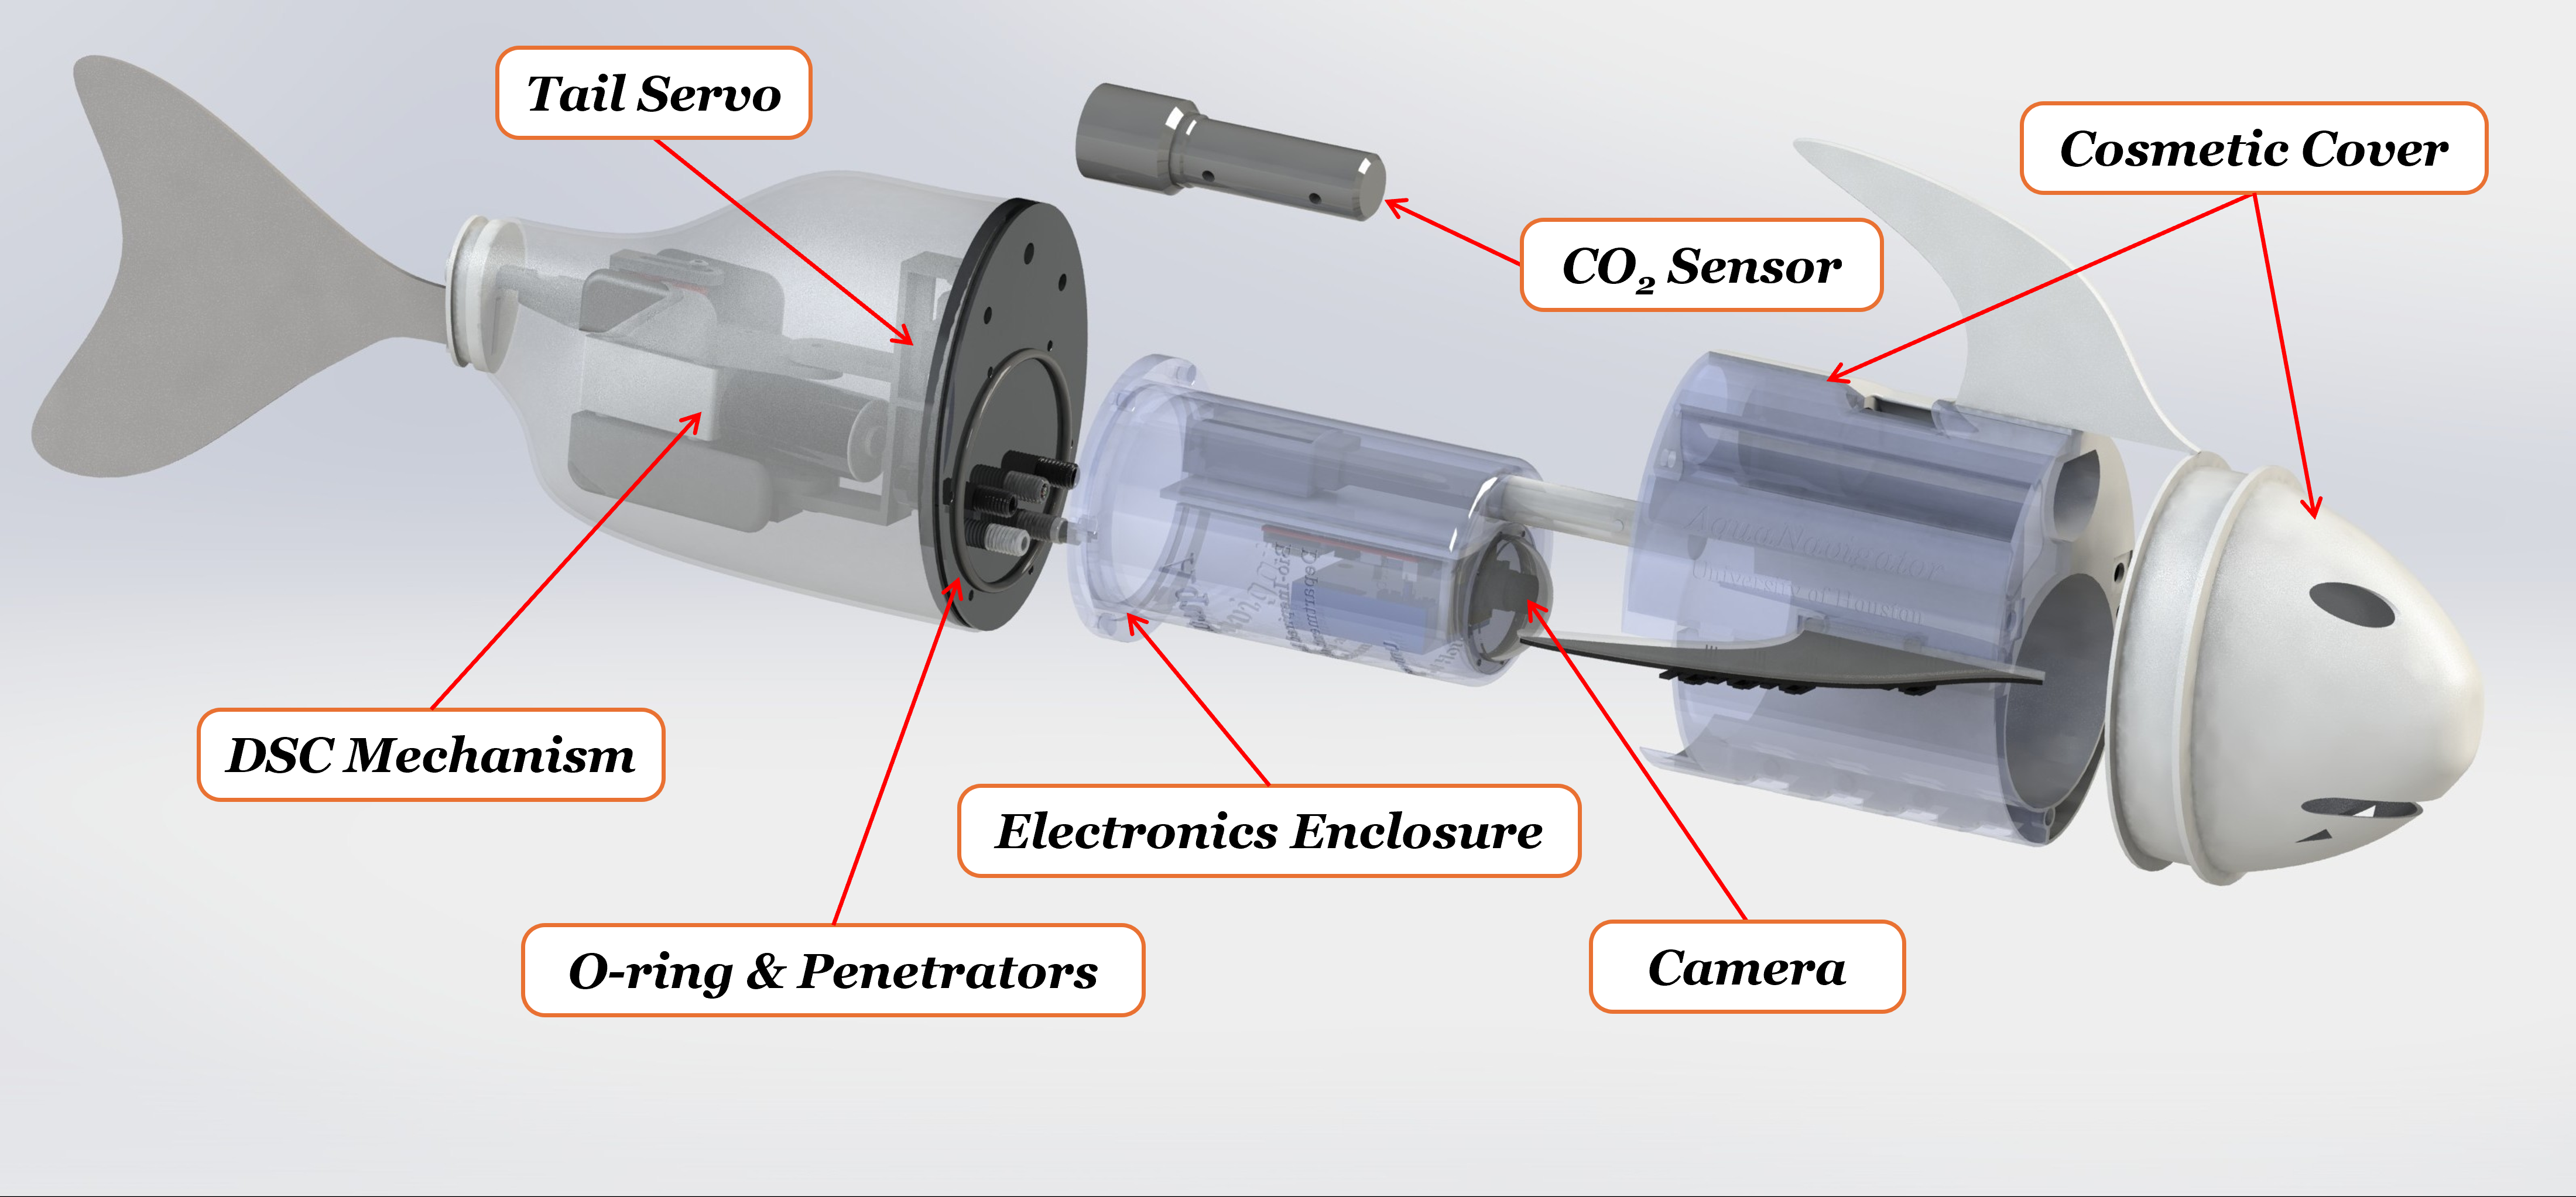
\includegraphics[width=0.6\textwidth]{Fig/CAD Model.png} 
    \caption{Annotated CAD model of AquaNavigator robotic fish.}
    \label{fig:cad_model}
\end{figure}


\section{DIFFUSION OF CO$_2$}
When CO$_2$ is leaked underwater, depending upon the source and shape of the leak point, its diffusion rate is affected by various factors. It is important to note, that any un-diffused CO$_2$ will rise to the surface and mix back with the atmospheric air, as where it was captured from. This $\rm{CO_2}$ which mixed in air is not real concern, rather the diffused $\rm{CO_2}$ is the one which can cause harm to the marine life. Under high static pressure of the water, the leaked CO$_2$ will dissolve in water, and a 3D cloud data of the diffused CO$_2$ can lead to the identification of the leak point.
In this scenario, it was important for us to study the diffusion of CO$_2$ in water, so an experimental setup was established in an indoor water tank of 1.2m x 1.2m x 1.2m dimensions. Remember this tank is different than the tank used for the testing of the robotic fish. A CO$_2$ cylinder is connected to a regulator and a flow meter to control the flow rate of CO$_2$. The outlet of the flow meter is connected to a pipe which is submerged in water. The pipe has a small hole at the bottom to simulate the leak point. This experimental setup is shown in Fig. \ref{fig:co2_setup}. 
\begin{figure}[ht]
    \centering
    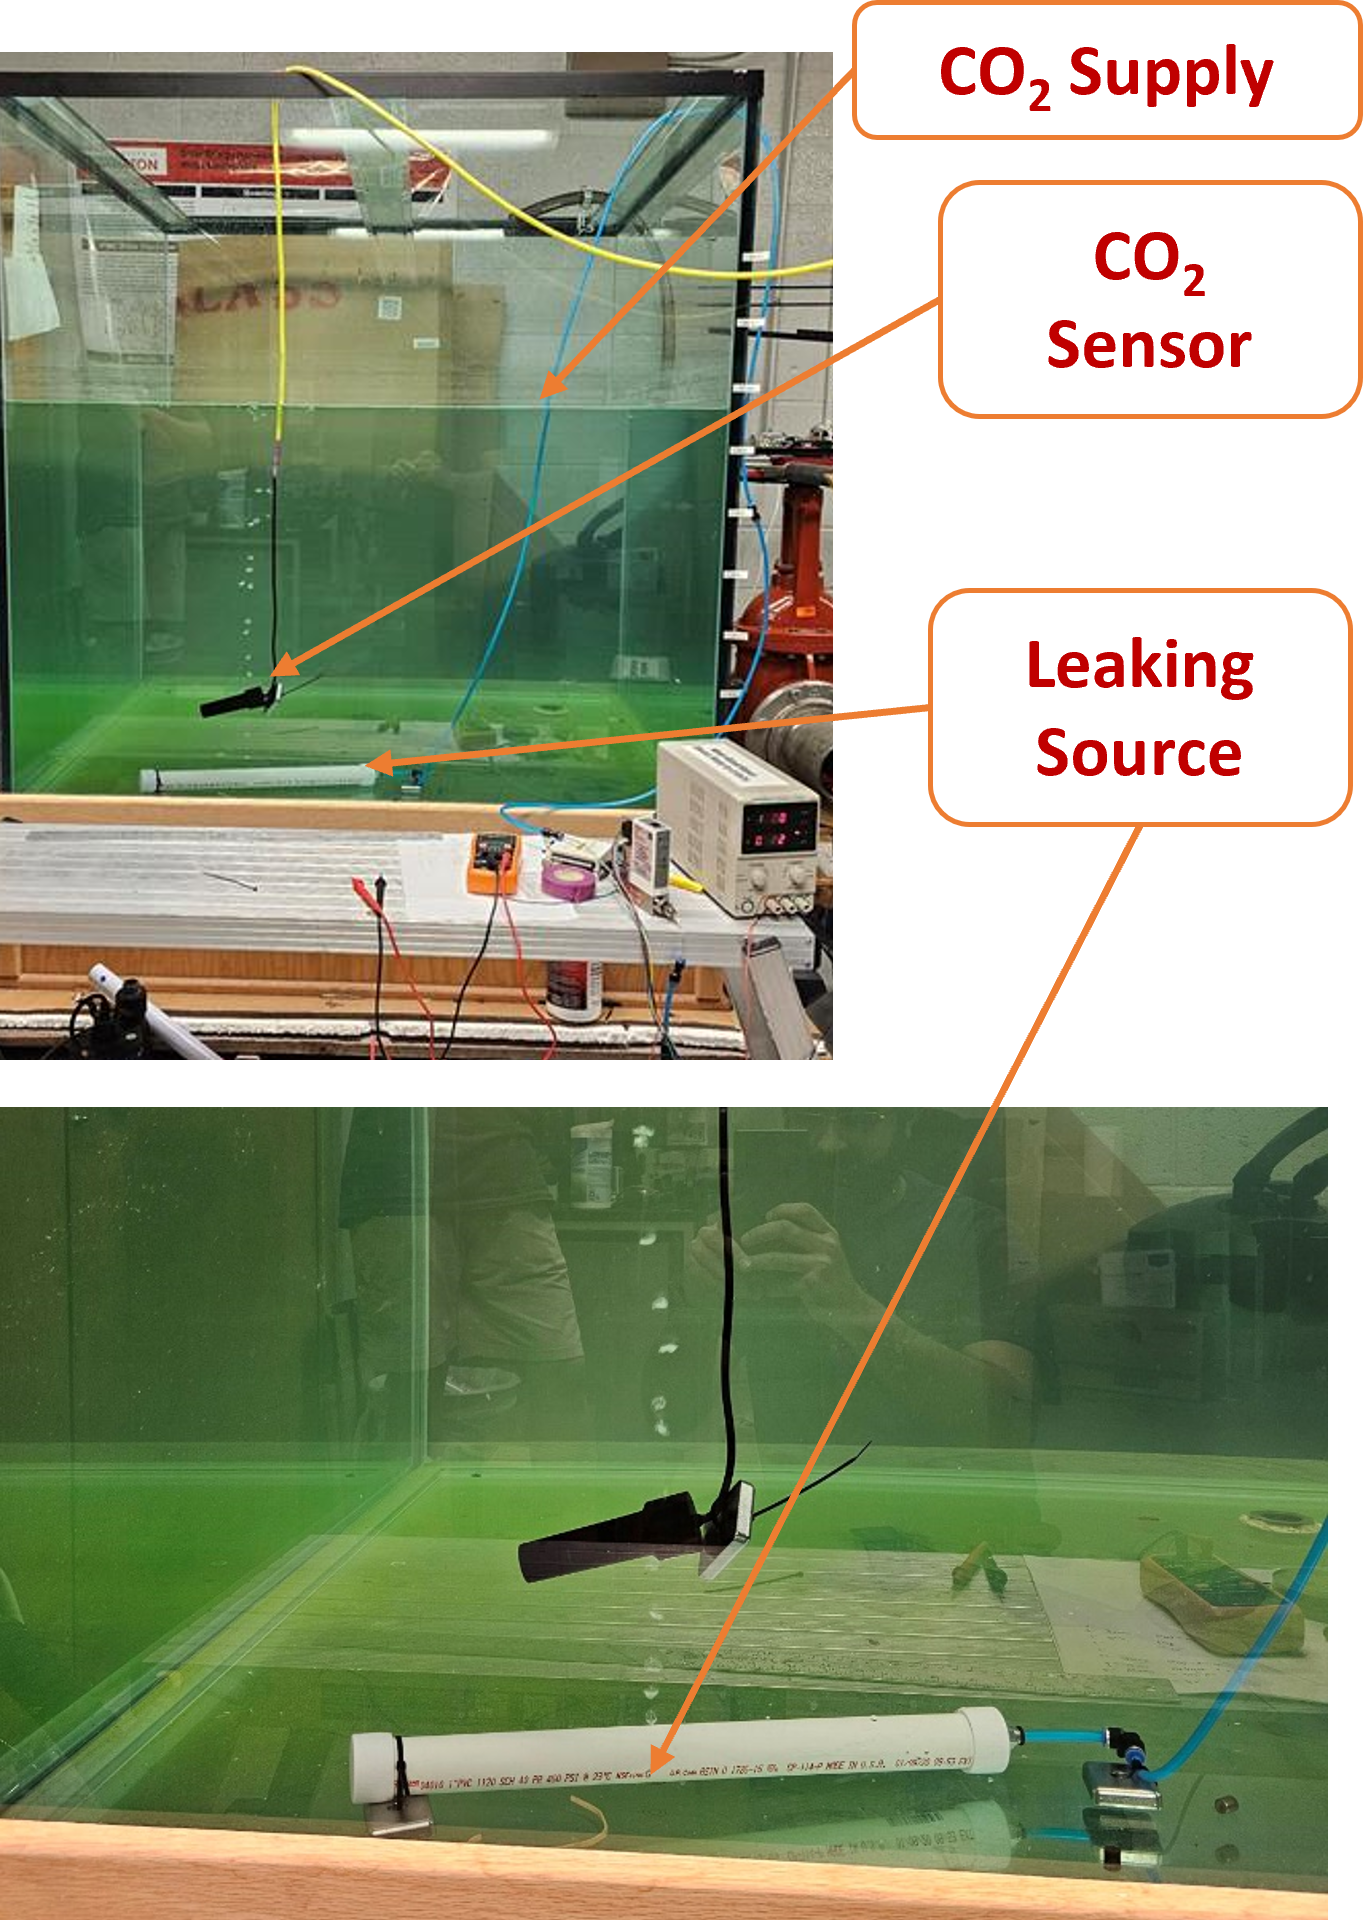
\includegraphics[width=0.48\textwidth]{Fig/DiffusionExperimentSetup.png} 
    \caption{Experimental setup for studying the diffusion of CO$_2$ in water.}
    \label{fig:co2_setup}   
\end{figure}
Provided that the Near Infrared (NIR) CO$_2$ sensor has a response time of 60 seconds, before turning on the leakage, the based line reading of the sensor was noted. The CO$_2$ leakage was turned on at a flow rate of 1 liter per minute (LPM) and the readings were noted at different depths and different horizontal distances from the leak point. The CO$_2$ readings were noted after every 5 minutes, to allow the sensor to stabilize. The CO$_2$ readings were noted at 3 different depths, 0.1m, 0.2m, 0.3m and 0.4m from the water surface, and at 5 different horizontal distances from the leak point, 0m, 0.1m, 0.2m and 0.3m. The CO$_2$ readings were noted for a total duration of 30 minutes. The experimental results are shown in Fig. \ref{fig:co2_results}. It can be observed that the CO$_2$ concentration is not highest near the leak point, rather it is highest at a certain distance from the leak point. This is due to the fact that the leaked CO$_2$ is in the form of bubbles, which rise to the surface and dissolve in water. As the bubbles rise, they dissolve in water and form carbonic acid, which lowers the pH of the water. The dissolved CO$_2$ then diffuses in water, leading to a higher concentration at a certain distance from the leak point. The experimental results also show that the CO$_2$ concentration decreases with increasing depth, as the static pressure of the water increases with depth, leading to a higher dissolution rate of CO$_2$ in water.
\begin{figure}[ht]
    \centering
    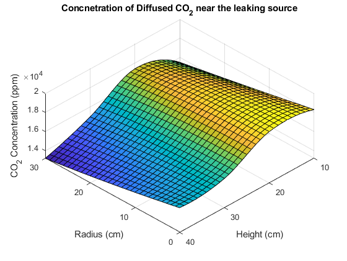
\includegraphics[width=0.6\textwidth]{Fig/DiffusionPlot.png} 
    \caption{Experimental results showing the diffusion of CO$_2$ in water at different depths and horizontal distances from the leak point.}
    \label{fig:co2_results}
\end{figure}

\section{CO$_2$ MONITORING SOFTWARE AND DATA COLLECTION}
A combined user-friendly software is developed to control the robotic fish and to monitor and record the sensed diffused CO$_2$ level in water. The software is developed in Python programming language and has a graphical user interface (GUI) to interact with the user. For the user's standpoint, the software has two main parts: (1) Manual Control of the robotic fish, and (2) Mission mode, which allows the user to set a predefined speed, depth rate, and curvature of the maneuvering path. With the mission mode, the robotic fish will move in a spiral path going downwards allowing it to scan a large area in water. The GUI of the software is shown in Fig. \ref{fig:software}.
\begin{figure}[ht]
    \centering
    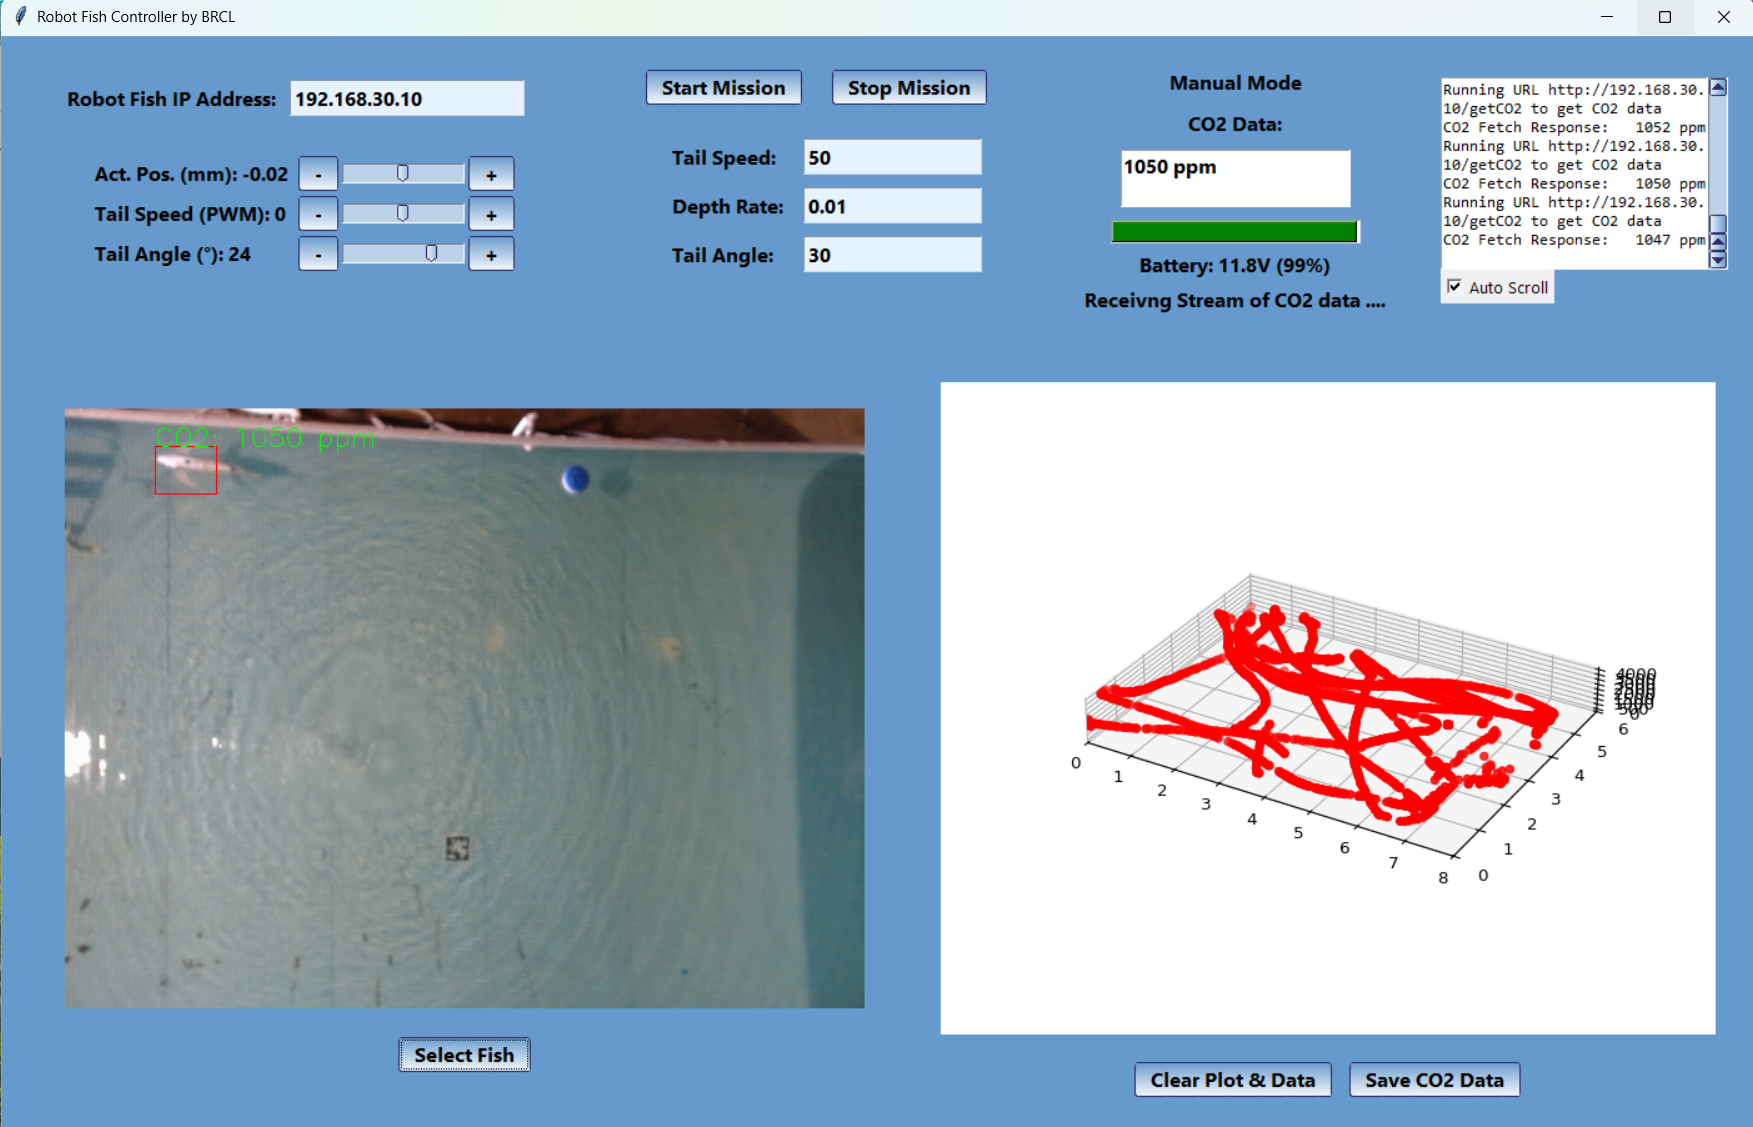
\includegraphics[width=0.6\textwidth]{Fig/CO2 GUI - Blue.png} 
    \caption{Graphical User Interface (GUI) of the developed software for controlling the robotic fish and monitoring the CO$_2$ levels in water.}
    \label{fig:software}    
\end{figure}

\subsection{Experimental Setup}
The experimental setup consists of an indoor water tank of dimensions 10 m x 5 m x 2 m, filled with about 70 percent of the height, with fresh water. An Red-Green-Blue (RGB) camera is mounted on the top of the water tank, which covers about 8 m x 6 m area of the water tank. The camera is connected to the computer and the software uses computer vision techniques to track the position of the robotic fish in the water tank. A CO$_2$ cylinder is connected to a regulator and a fixed leak rate was set from the tank. The outlet of the regulator is connected to a 2 inch diameter pipe which is submerged in water and has a small hole at the bottom to simulate the leak point as shown in Fig. \ref{fig:leaksource}. The $\rm{CO_2}$ would come of the leakage holes in the form of bubbles, rise to the surface and dissolve in air. As evident from the lab experiment in the previous section, some of this $\rm{CO_2}$ will dissolve in water and diffuse in water. The ratio of $\rm{CO_2}$ which dissolves in water depends upon the static pressure of the water, flow rate of the leakage, temperature of the water and other factors. The purpose of this study to use the data analysis techniques to localize the leak point without considering all those complex parameters.

The experimental setup consists of an indoor water tank of dimensions 10 m x 5 m x 2 m, filled with about 70 percent of the height, with fresh water. An Red-Green-Blue (RGB) camera is mounted on the top of the water tank, which covers about 8 m x 6 m area of the water tank. The camera is connected to the computer and the software uses computer vision techniques to track the position of the robotic fish in the water tank. A CO$_2$ cylinder is connected to a regulator and a fixed leak rate was set from the tank. The outlet of the regulator is connected to a 2 inch diameter pipe which is submerged in water and has a small hole at the bottom to simulate the leak point as shown in Fig. \ref{fig:leaksource}. The $\rm{CO_2}$ would come of the leakage holes in the form of bubbles, rise to the surface and dissolve in air. As evident from the lab experiment in the previous section, some of this $\rm{CO_2}$ will dissolve in water and diffuse in water. The ratio of $\rm{CO_2}$ which dissolves in water depends upon the static pressure of the water, flow rate of the leakage, temperature of the water and other factors. The purpose of this study to use the data analysis techniques to localize the leak point without considering all those complex parameters.
\begin{figure}[ht]
    \centering
    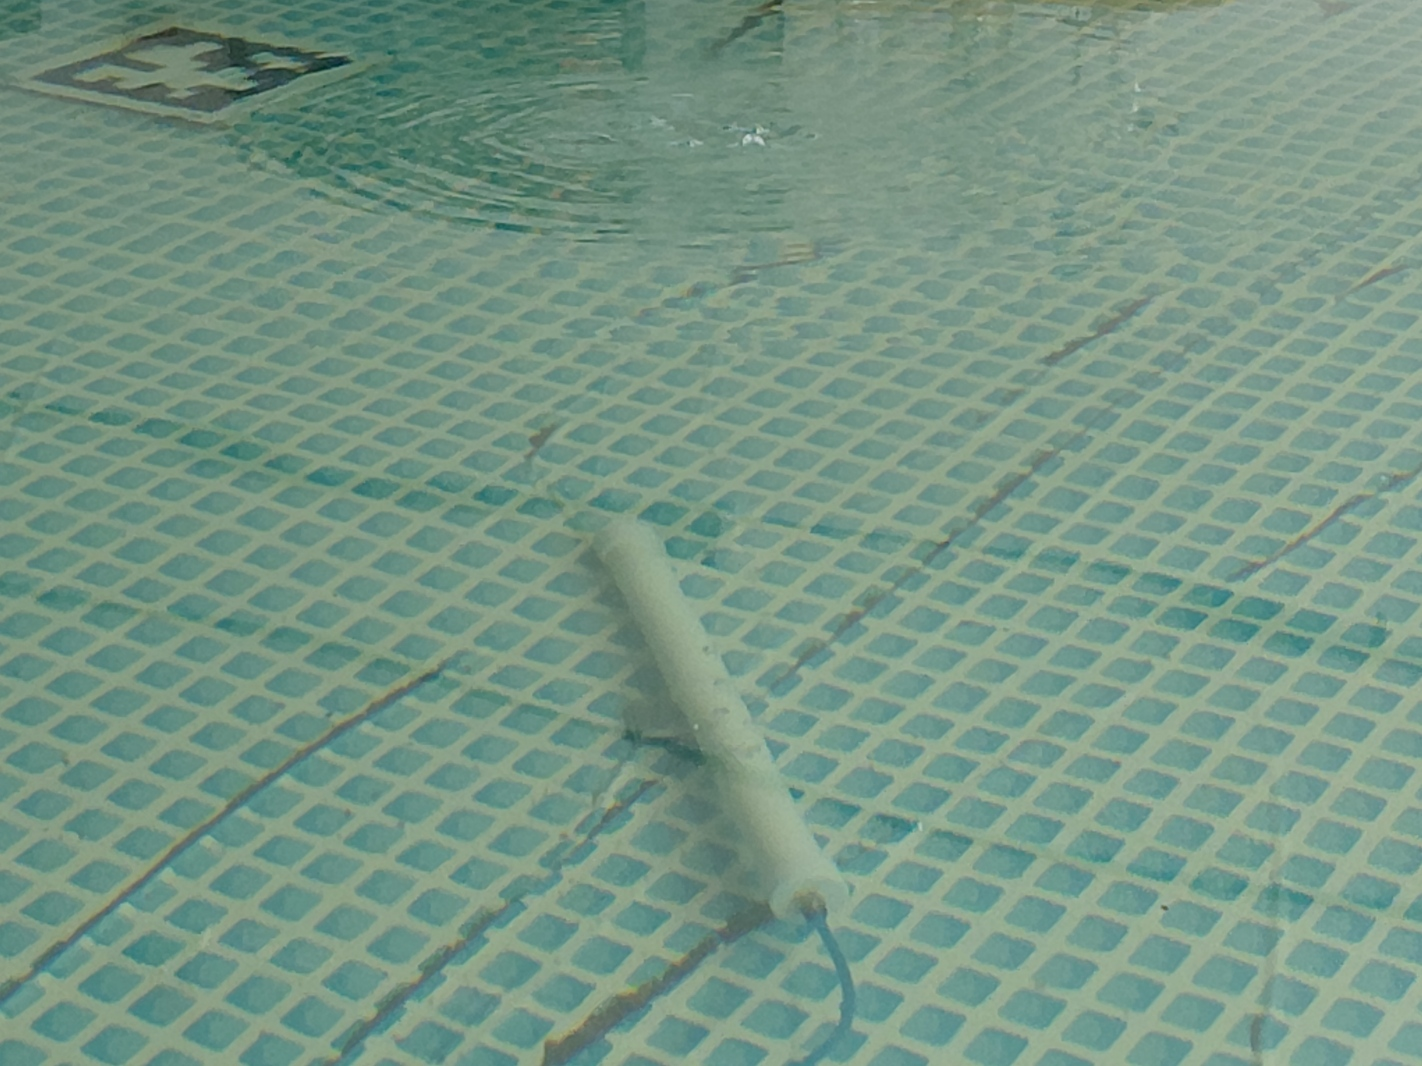
\includegraphics[width=0.6\textwidth]{Fig/Leak Source.jpg} 
    \caption{CO$_2$ leakage source setup in the water tank.}
    \label{fig:leaksource}
\end{figure}

The robotic fish is placed on the surface of the water, and been controlled manually from the software. The initial detection of the robotic fish is done by the human assistance, and then the visual tracker keeps the postion of the robotic fish using optical flow techniques. Through out the manual operation of the robotic fish, the diffused CO$_2$ levels are sensed and being sent to the host computer and been live plotted in the software. The complete experimental setup is shown in Fig. \ref{fig:exp_setup}.
\begin{figure}[ht]
    \centering
    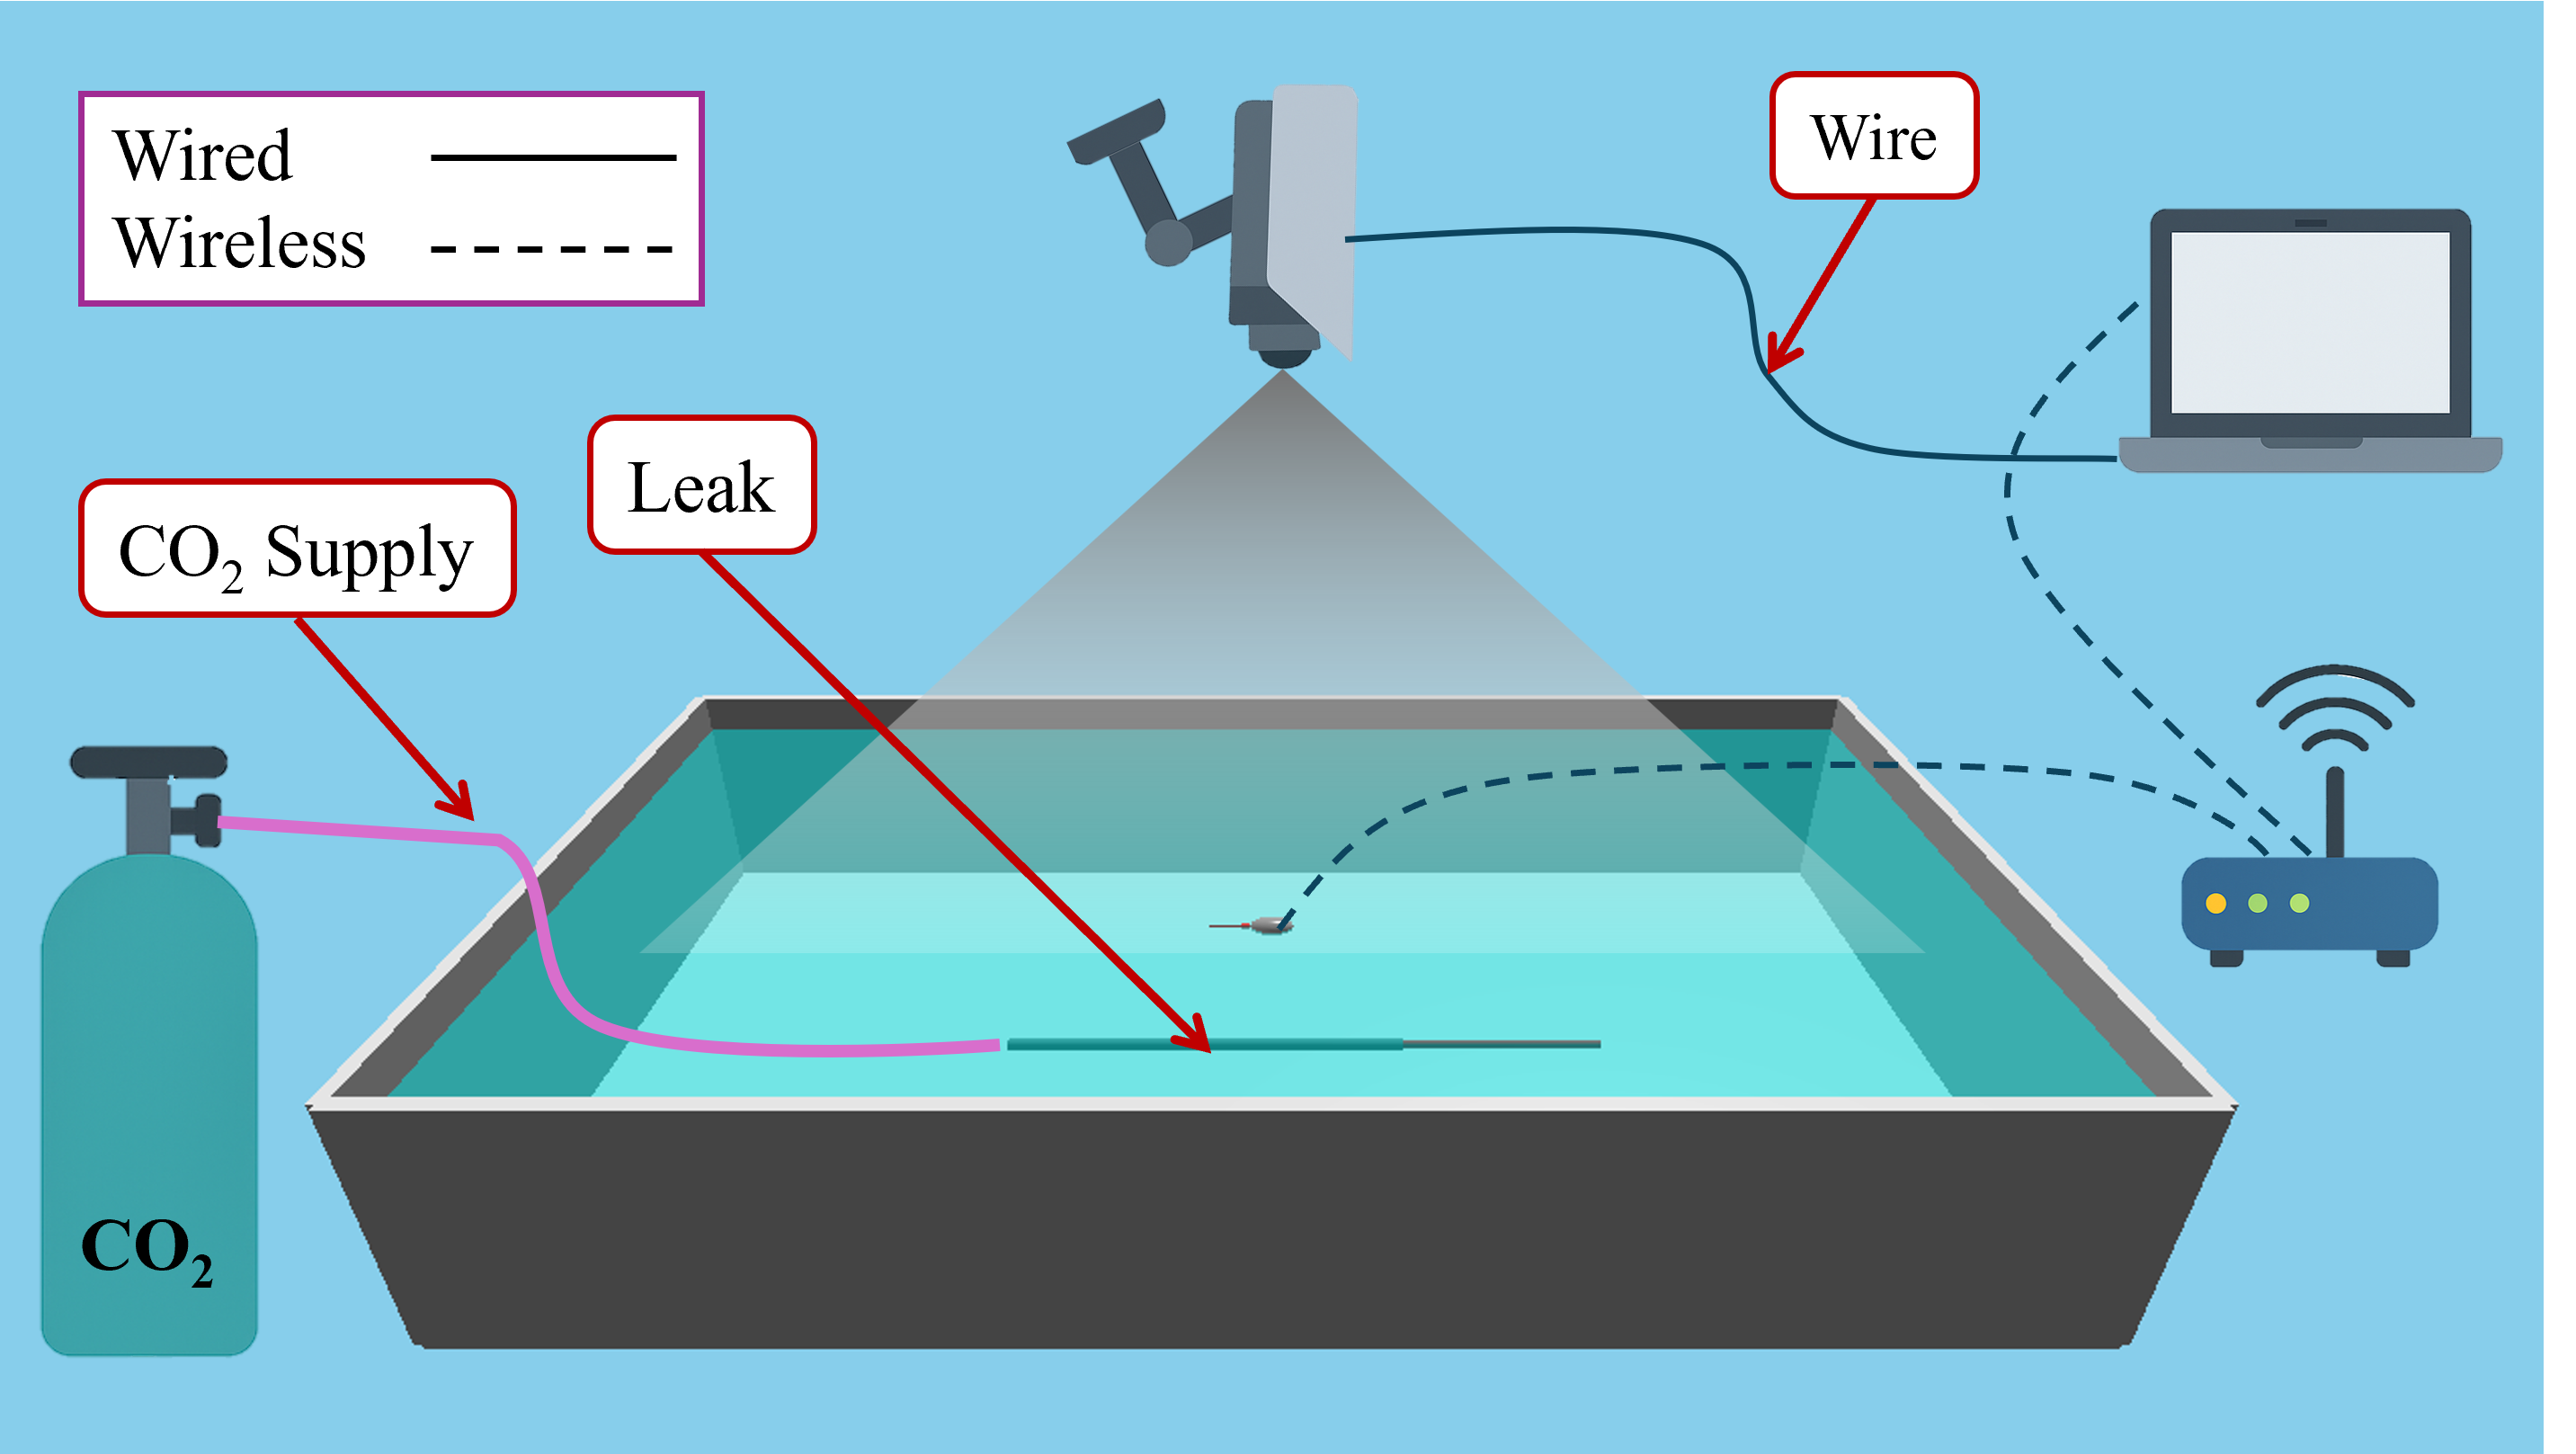
\includegraphics[width=0.6\textwidth]{Fig/exp-setup.png} 
    \caption{Complete experimental setup for testing the robotic fish and monitoring the diffused CO$_2$ levels in water.}
    \label{fig:exp_setup}
\end{figure}

\subsection{Communication}
The robotic fish is equipped by a ESP32-C3 microcontroller, which has built-in wireless IEEE 802.11 (Wi-Fi). For the demonstration purposes, it is good enough to communicate with this wireless in an indoor water tank. However, for the real-world applications, a more robust communication system is required, such as very low frequency (VLF) radio waves or acoustic communication. The idea remains the same, when the robotic fish is not able to successfully send the data through wireless communication, it will store the data in its internal memory and send it when it is back in the range of communication. At the minimum, the robotic fish will be able to send the data when it surfaces. Other than communication frequency, the data sending mechanism will remain the same.\\
The robotic fish and the computer communicate over a TCP/IP socket connection. The robotic fish acts as a server and the computer acts as a client. The computer sends control commands to the robotic fish, and the robotic fish sends back the status and sensor data. The communication protocol is simple and easy to implement, making it suitable for real-time applications. The socket requests are sent as scheduled tasks for different functionalities, such as sending control commands, receiving status updates, and receiving sensor data. When the computer software does not receive any response from the robotic fish within a certain time, it assumes that the connection is lost and intimates the user. If the robotic fish does not receive any command from the computer within a certain time, it assumes that the connection is lost, keeps storing the sensor data, and stops moving to avoid any accidents, unless it is in mission mode. Fig. \ref{fig:exp_setup} shows the communication flow between the robotic fish and the computer.
\subsection{Geo tagging of CO$_2$ Data}
We know the limitation of the Global Positioning System (GPS) in an indoor environment, and it is not practical to use GPS in indoors. So, for the purpose of this research, a camera is mounted on the top of the water tank to provide the localization of the robotic fish. The camera is connected to the computer and the software uses computer vision techniques to track the position of the robotic fish in the water tank. The camera captures the images of the water tank and processes them to detect the robotic fish. The position of the robotic fish is then calculated based on its location in the image. The software uses OpenCV library for image processing and computer vision tasks. The position of the robotic fish is then used to tag the CO$_2$ data with its corresponding location in the water tank. Irrespective of the mission mode, the software will always keep plotting the diffused CO$_2$ levels corresponding to its position in the 3D plot in the GUI. The 3D plot is updated in real-time as the robotic fish moves in the water tank. The user can also save the CO$_2$ data with its corresponding location in a CSV file for further analysis. The 3D plot of the diffused CO$_2$ levels in water tank is shown in Fig. \ref{fig:3dplot}. The data analysis of this data is further discussed in the next section.
\begin{figure}
    \centering
    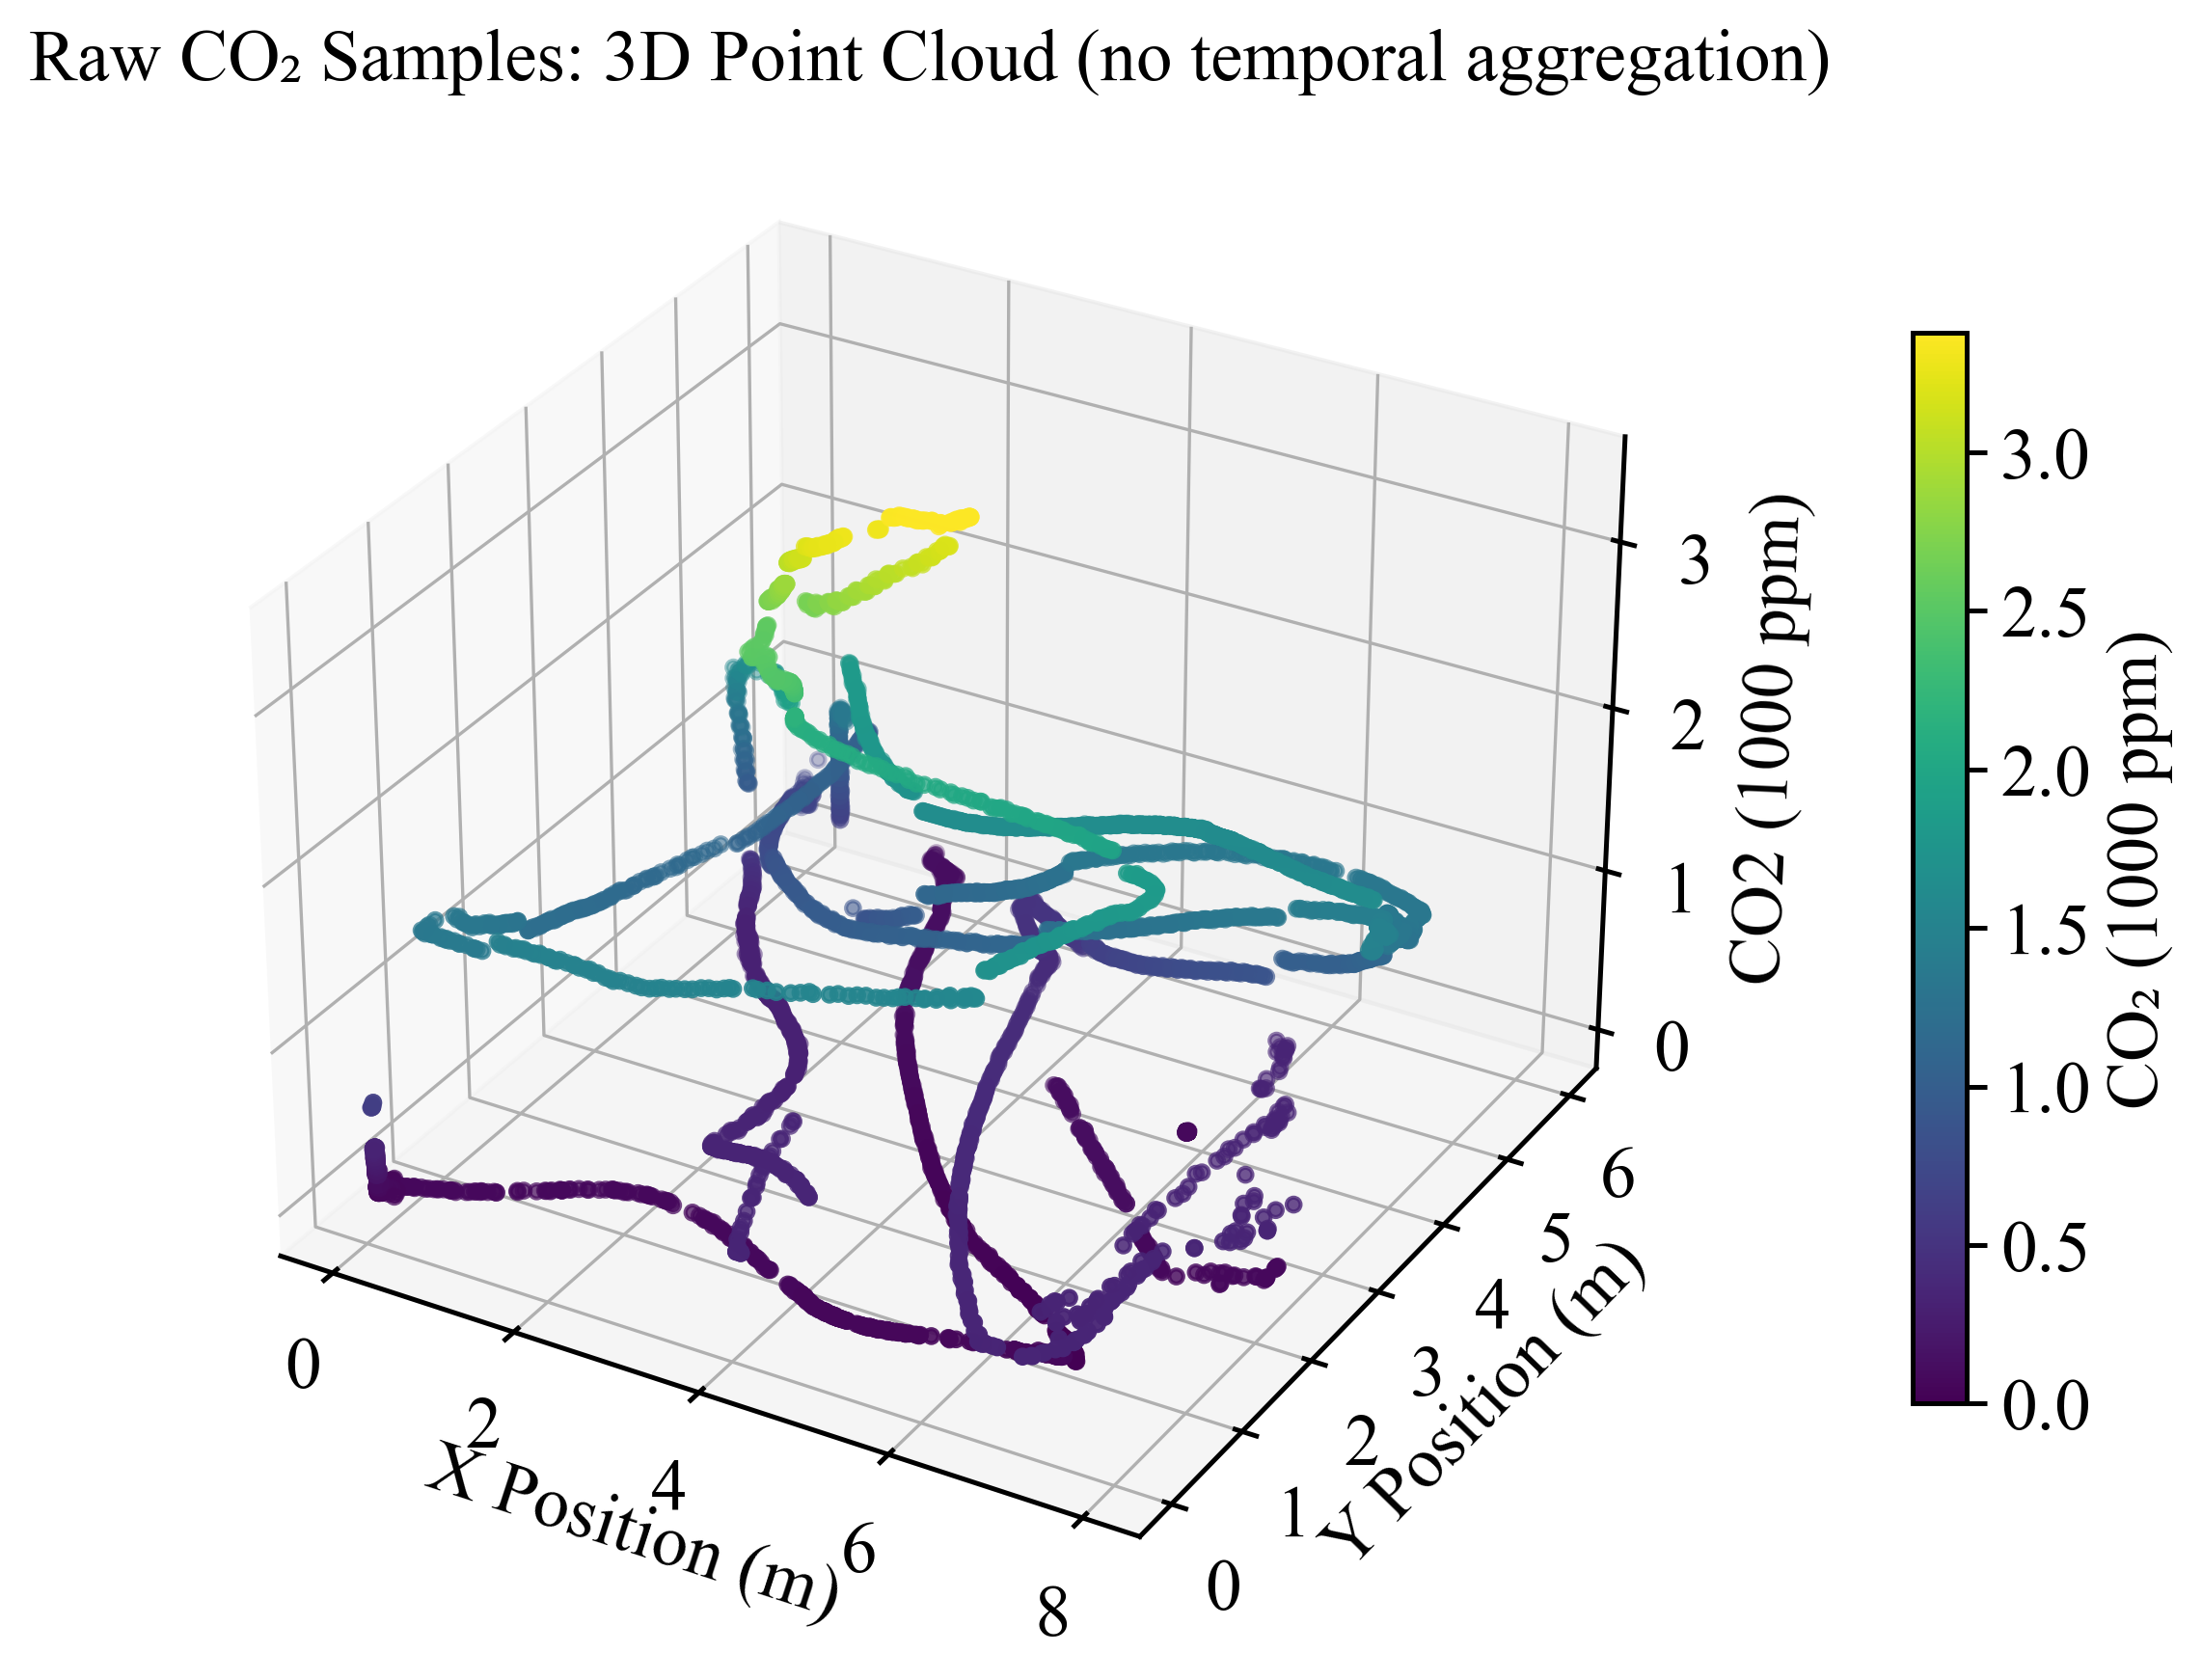
\includegraphics[width=0.6\textwidth]{Fig/01_raw_3d_scatter.png} 
    \caption{3D plot showing the diffused CO$_2$ levels in water tank. The color bar shows the CO$_2$ concentration in ppm.}
    \label{fig:3dplot}
\end{figure}

\section{RESULTS AND DISCUSSION}
The data of diffused CO$_2$ levels in the water tank is collected by the robotic fish and tagged with its corresponding position in the tank. Although the data is collected over time, with each data point being approximately 0.1 seconds apart, the processing of the full spatiotemporal dataset is computationally expensive. Furthermore, considering that the time response of state-of-the-art dissolved CO$_2$ sensors is on the order of 60 seconds, it is reasonable to assume that the data collected over a short period of time can be treated as quasi-steady. Hence, for the purpose of the present analysis, the data is regarded as spatial, and the temporal component is ignored. This assumption allows the use of spatial interpolation and binning techniques to visualize and analyze the CO$_2$ diffusion pattern. If the leakage source can be localized without explicitly modeling temporal evolution, the approach provides an efficient means to identify the leak origin.\\
\subsection{Spatial Data Analysis}
To obtain a spatially continuous representation of the CO$_2$ field, the raw measurements are discretized into a uniform 2D grid, and the average CO$_2$ concentration within each cell is computed to generate a binned heatmap. The mean concentration $\bar{C}(x_i, y_j)$ in each grid cell centered at $(x_i, y_j)$ is given by
\begin{align}
\bar{C}(x_i, y_j)
&= \frac{
    \displaystyle \sum_{n=1}^{N} C_n \,
    \delta_{ij}(x_n, y_n)
}{
    \displaystyle \sum_{n=1}^{N} \delta_{ij}(x_n, y_n)
}
\label{eq:binned_heatmap} \\[1em]
\delta_{ij}(x_n, y_n) &=
\begin{cases}
1, & x_n \in [x_i - \tfrac{\Delta x}{2},\, x_i + \tfrac{\Delta x}{2}), \\
   & y_n \in [y_j - \tfrac{\Delta y}{2},\, y_j + \tfrac{\Delta y}{2}), \\
0, & \text{otherwise}.
\end{cases}
\nonumber
\end{align}
Here, $C_n$ denotes the CO$_2$ concentration measured at location $(x_n, y_n)$, and $(\Delta x, \Delta y)$ are the grid spacings in the $x$ and $y$ directions, respectively. The indicator function $\delta_{ij}$ assigns each measurement to the corresponding grid cell based on its spatial coordinates. The resulting two-dimensional heatmap, shown in Fig.~\ref{fig:heatmap}, captures the spatial distribution of CO$_2$ concentration within the water tank. It can be observed that the CO$_2$ concentration is highest near the leak point, which is expected due to the localized source. Other regions with elevated concentrations may correspond to zones of CO$_2$ diffusion and mixing within the water tank. This method is the computationally most effective, but may not be very accurate about estimating the leak point. As seen in the figure, the leak point is detected near (3.5, 4).
\begin{figure}
    \centering
    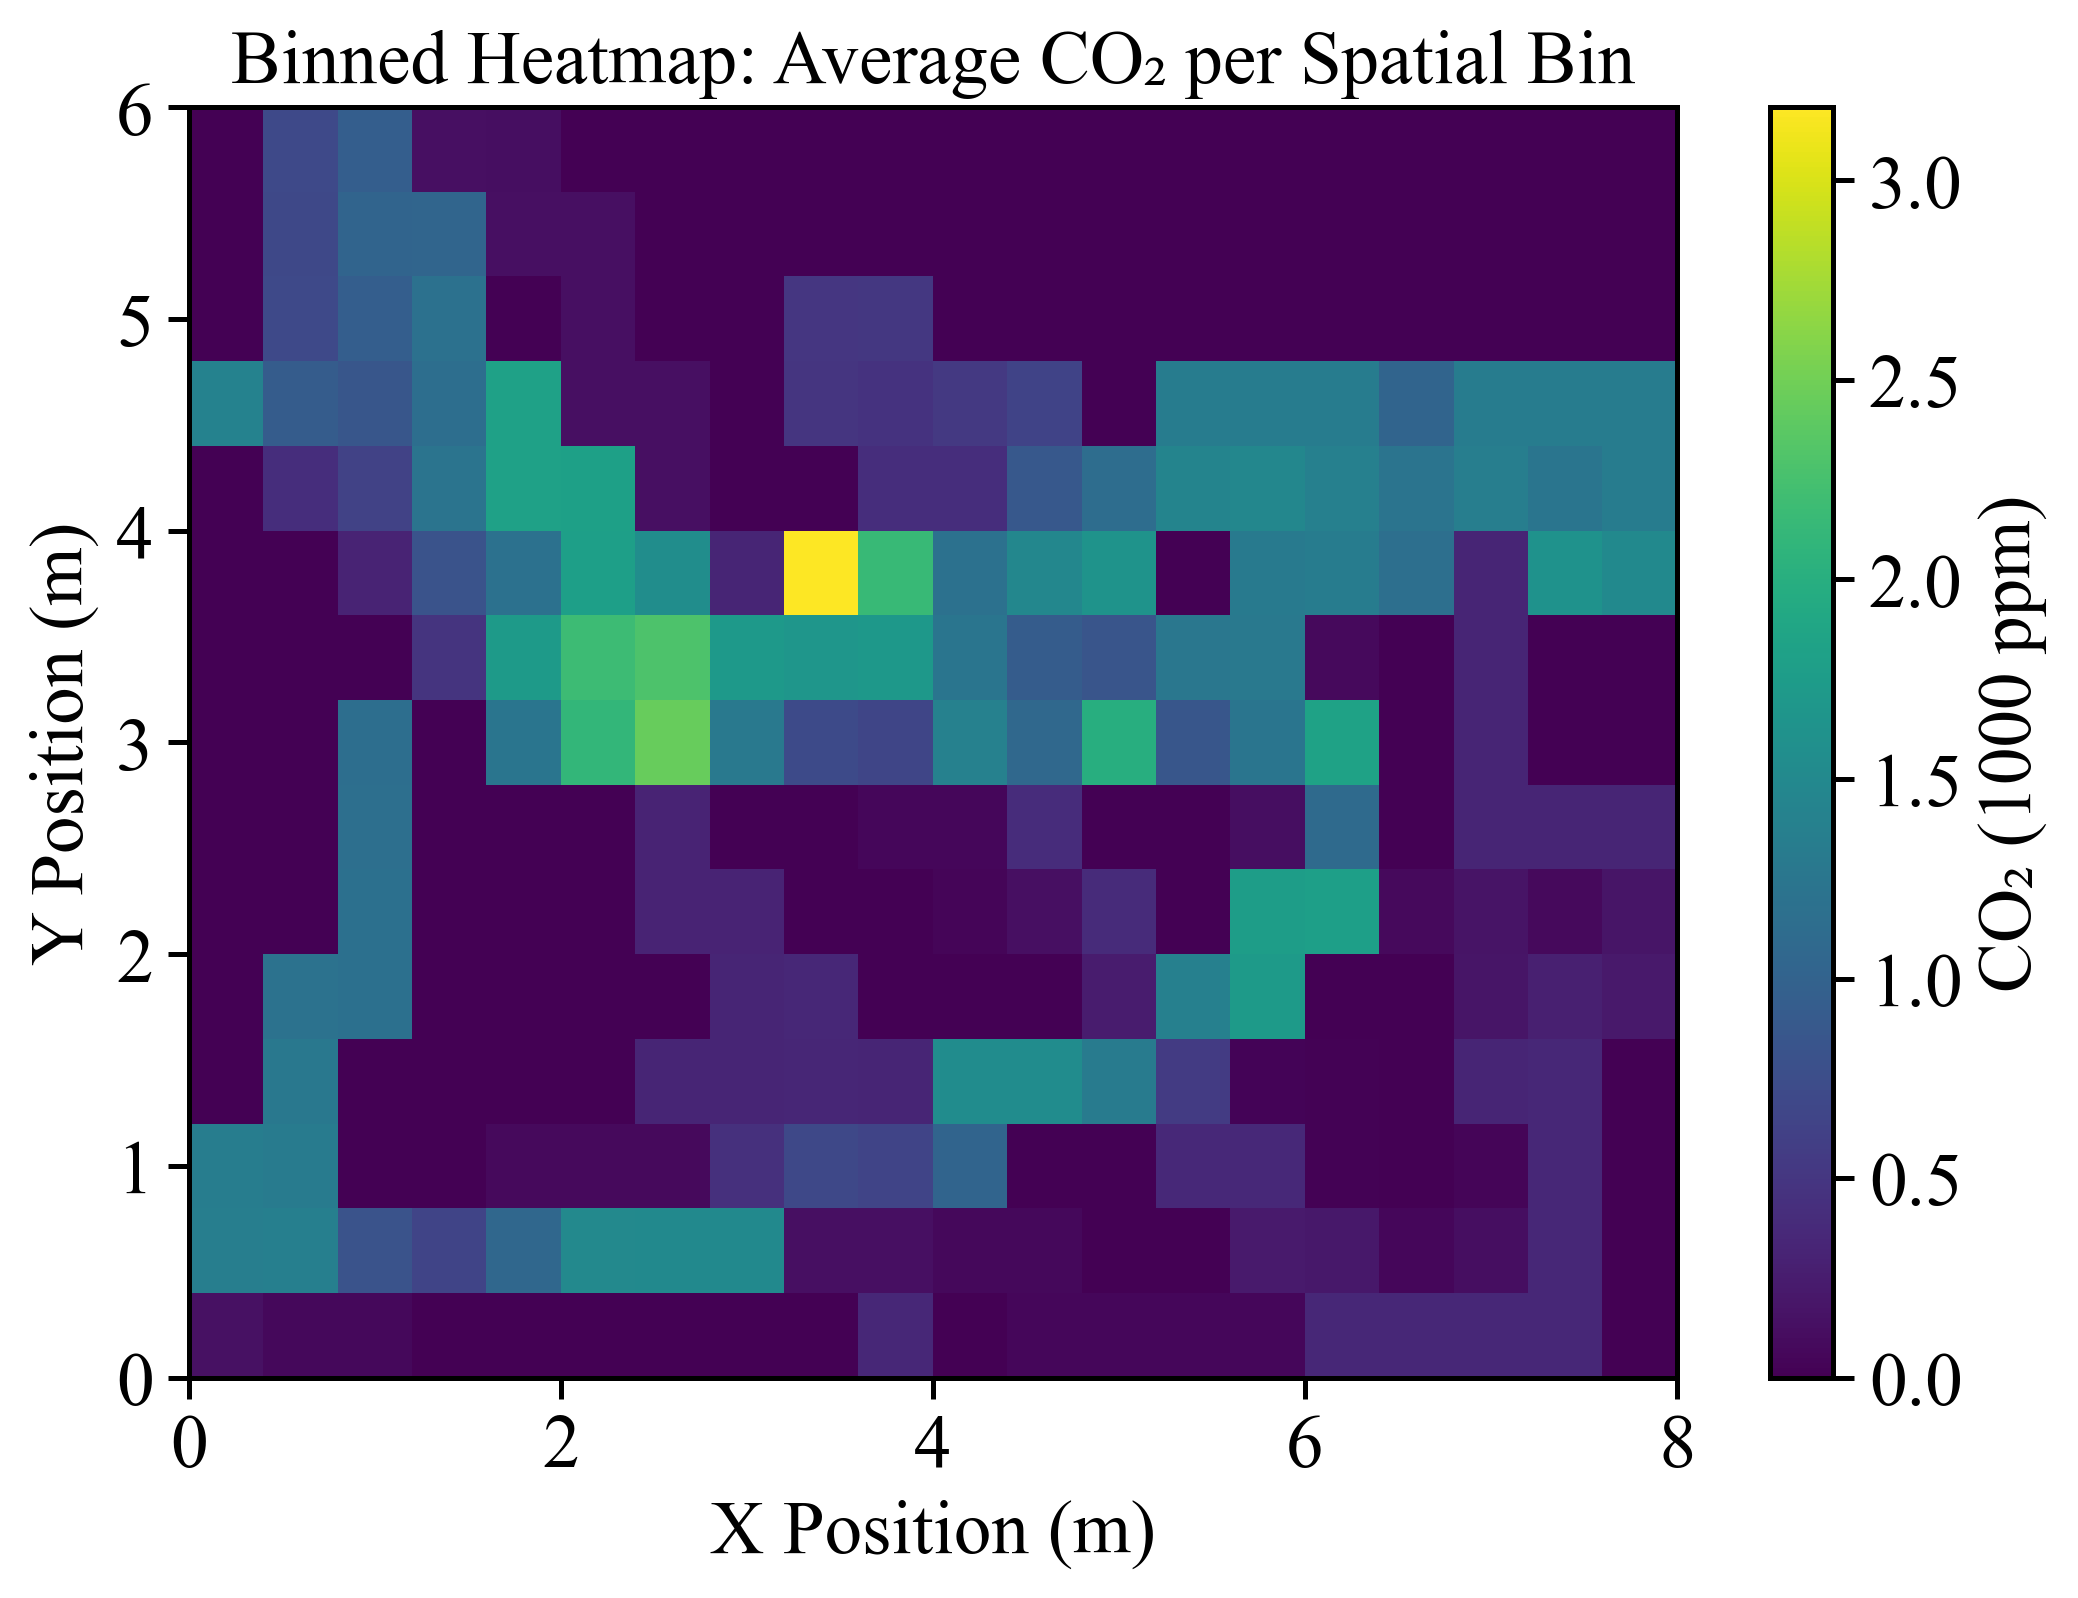
\includegraphics[width=0.6\textwidth]{Fig/02_binned_heatmap.png} 
    \caption{2D heatmap showing the diffused CO$_2$ levels in water tank, with a grid size of 0.4m x 0.4m.}
    \label{fig:heatmap}
\end{figure}
The scattered CO$_2$ measurements $\{(x_n, y_n, C_n)\}_{n=1}^N$ were interpolated onto a regular grid 
$(x_i, y_j)$ using piecewise linear interpolation. 
The interpolated field $C_g(x_i, y_j)$ is given by
\begin{equation}
C_g(x_i, y_j)
= \sum_{n=1}^{N} \lambda_n(x_i, y_j)\, C_n,
\qquad
\text{with} \quad
\sum_{n=1}^{N} \lambda_n(x_i, y_j) = 1,
\label{eq:linear_interp}
\end{equation}
where the interpolation weights $\lambda_n(x_i, y_j)$ are the barycentric coordinates of the point $(x_i, y_j)$ with respect to the Delaunay triangle enclosing it.
For grid points lying outside the convex hull of the sampled positions, 
the nearest‐neighbor interpolation is used to assign a value:
\begin{equation}
C_g^{\text{filled}}(x_i, y_j)
=
\begin{cases}
C_g(x_i, y_j), & (x_i, y_j) \in \Omega_{\text{hull}}, \\[3pt]
C_{n^*}, & (x_i, y_j) \notin \Omega_{\text{hull}},
\end{cases}
\label{eq:fill_nearest}
\end{equation}
where $\Omega_{\text{hull}}$ denotes the convex hull of the measurement locations 
and $n^*$ is the index of the nearest sample point.
\begin{figure}
    \centering
    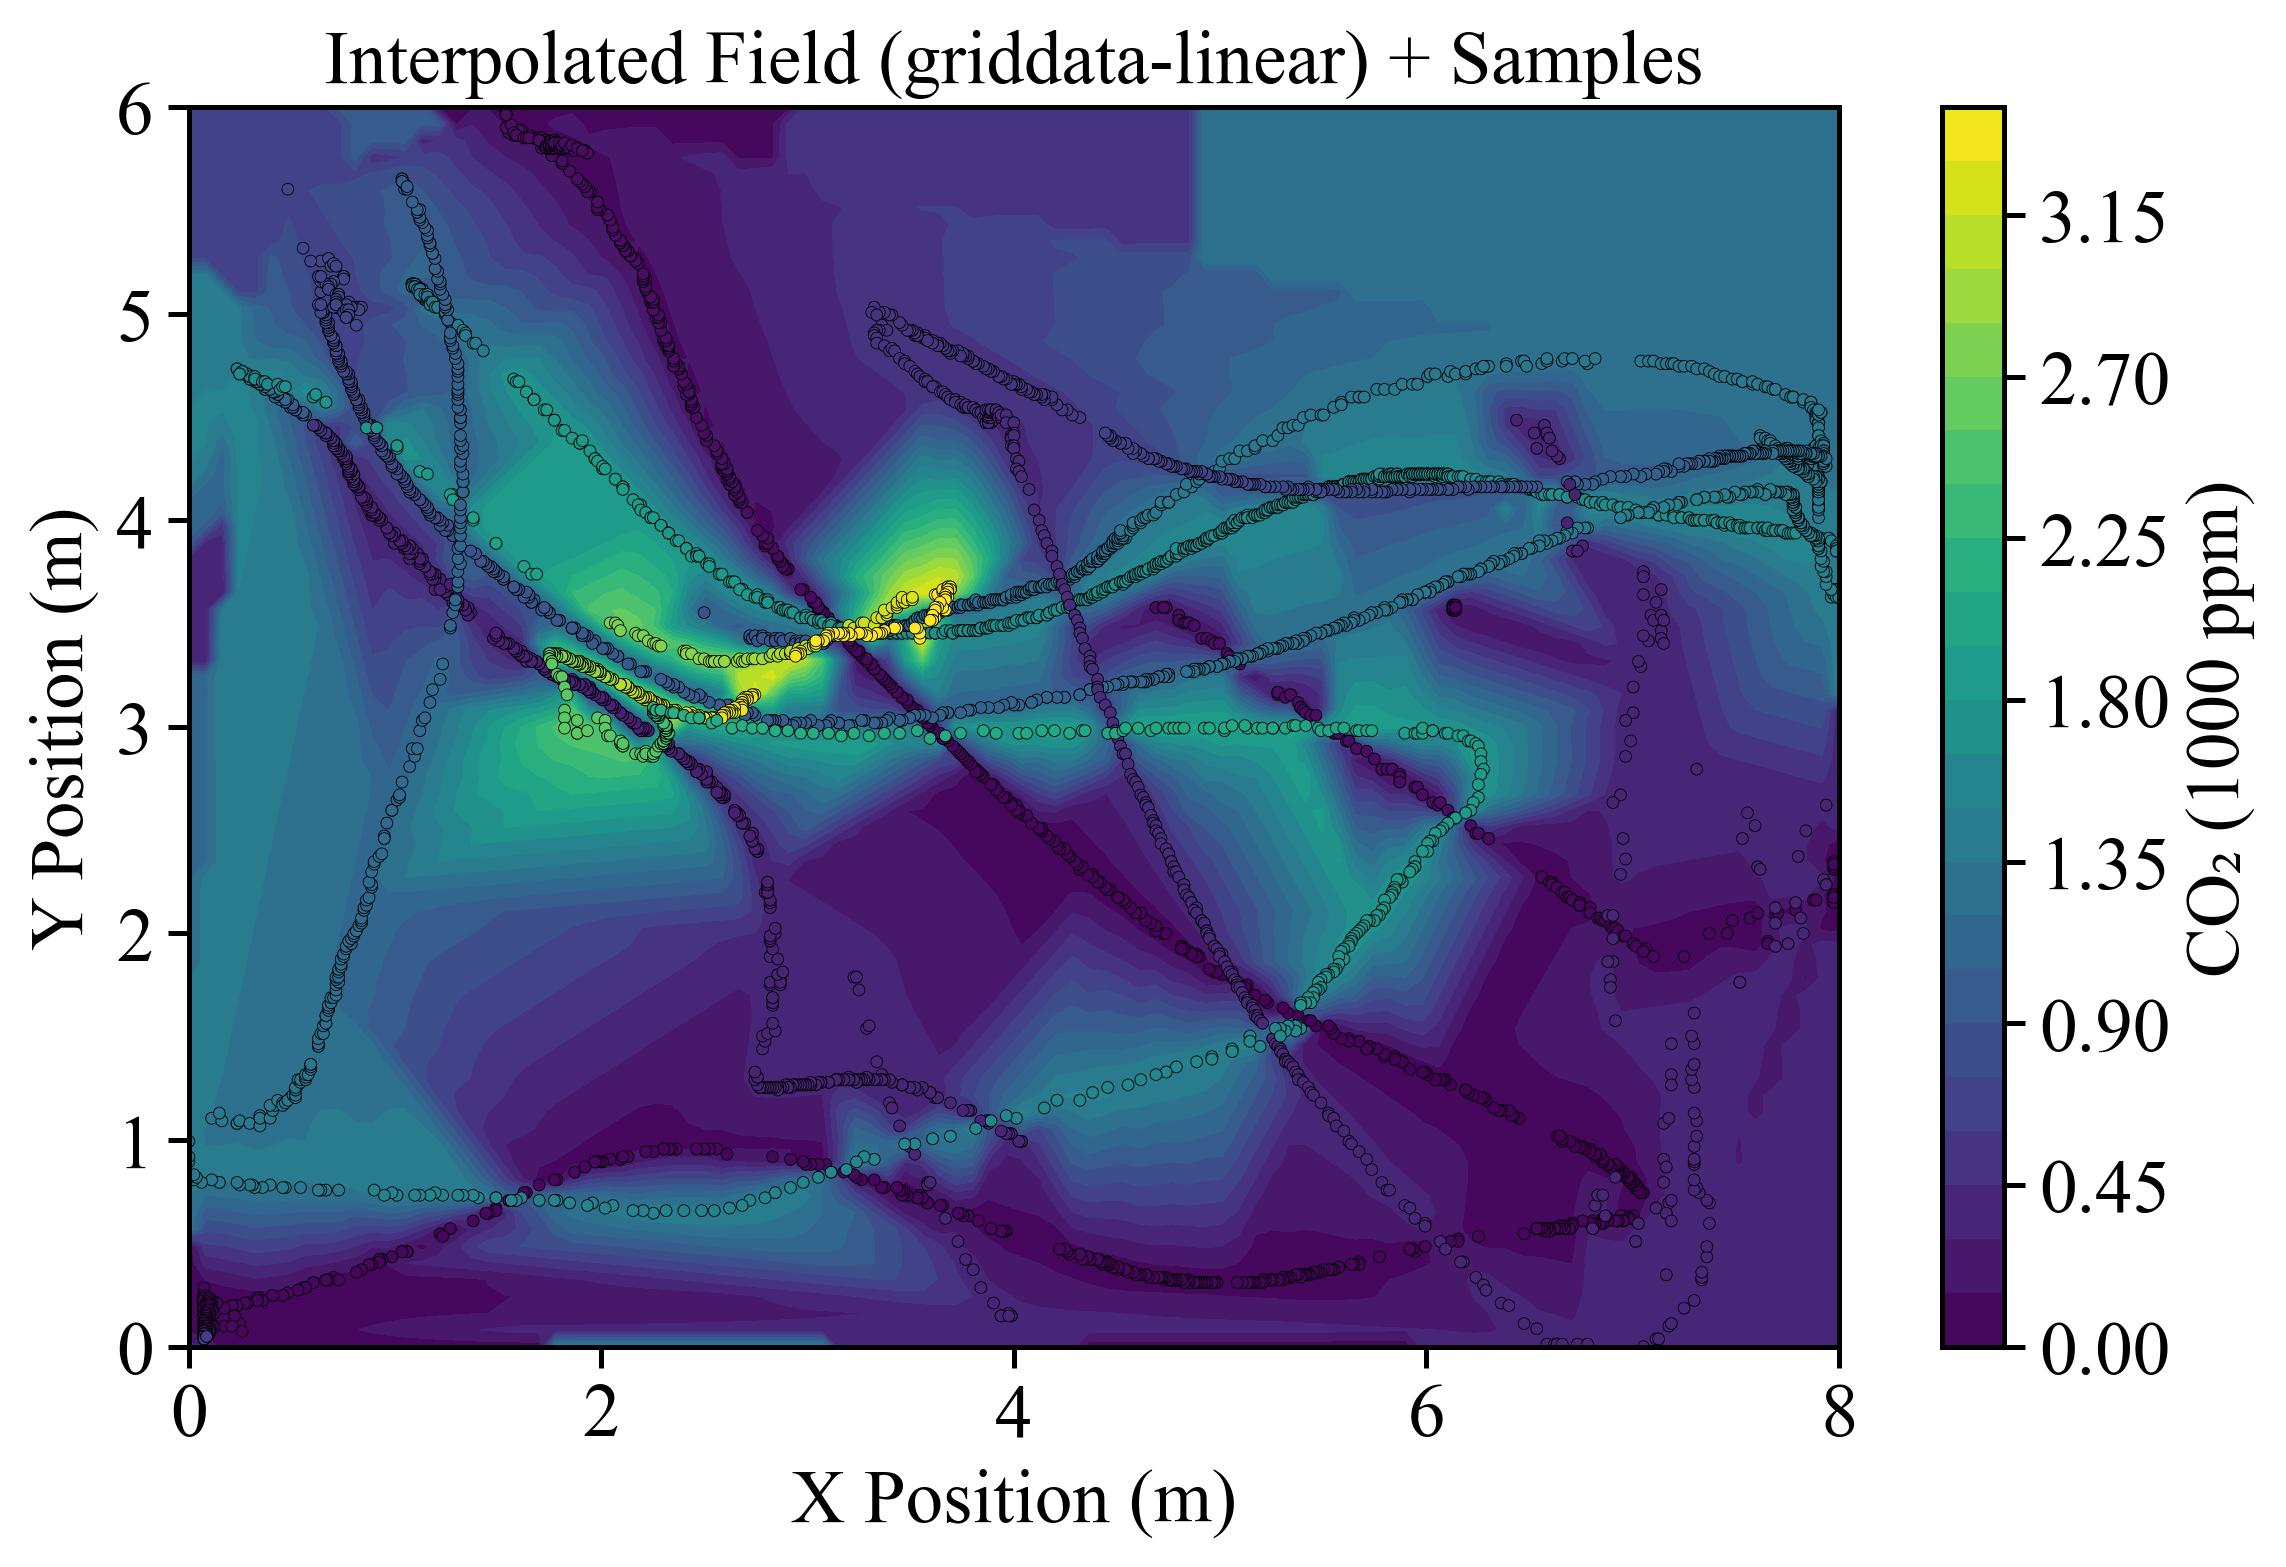
\includegraphics[width=0.6\textwidth]{Fig/03_griddata_linear.png} 
    \caption{Linear and nearest interpolation of the diffused CO$_2$ levels in water tank}
    \label{fig:interpolation}
\end{figure}

More for visual purposes, and less for direct leak localization, a radial basis function (RBF) interpolation is also applied to the scattered CO$_2$ measurements. 
The interpolated field $C_r(x_i, y_j)$ is expressed as
\begin{equation}
C_r(x_i, y_j) = \sum_{n=1}^{N} w_n \, 
\phi\!\left( \big\| (x_i, y_j) - (x_n, y_n) \big\| \right),
\label{eq:rbf_field}
\end{equation}
where $\phi(r)$ is a radial basis function, and the coefficients $w_n$ are determined by enforcing the interpolation condition 
$C_r(x_n, y_n) = C_n$ for all $n = 1, \dots, N$. 
A commonly used choice for $\phi(r)$ is the Gaussian kernel:
\begin{equation}
\phi(r) = \exp\!\left[-\left(\frac{r}{\epsilon}\right)^{2}\right],
\label{eq:rbf_gaussian}
\end{equation}
where $\epsilon$ is a shape parameter controlling the smoothness of the interpolation. The resulting RBF‐interpolated field, shown in Fig.~\ref{fig:rbf}, provides a smooth and visually continuous representation of the CO$_2$ concentration across the water tank, highlighting diffusion patterns while suppressing small‐scale measurement noise.
\begin{figure}
    \centering
    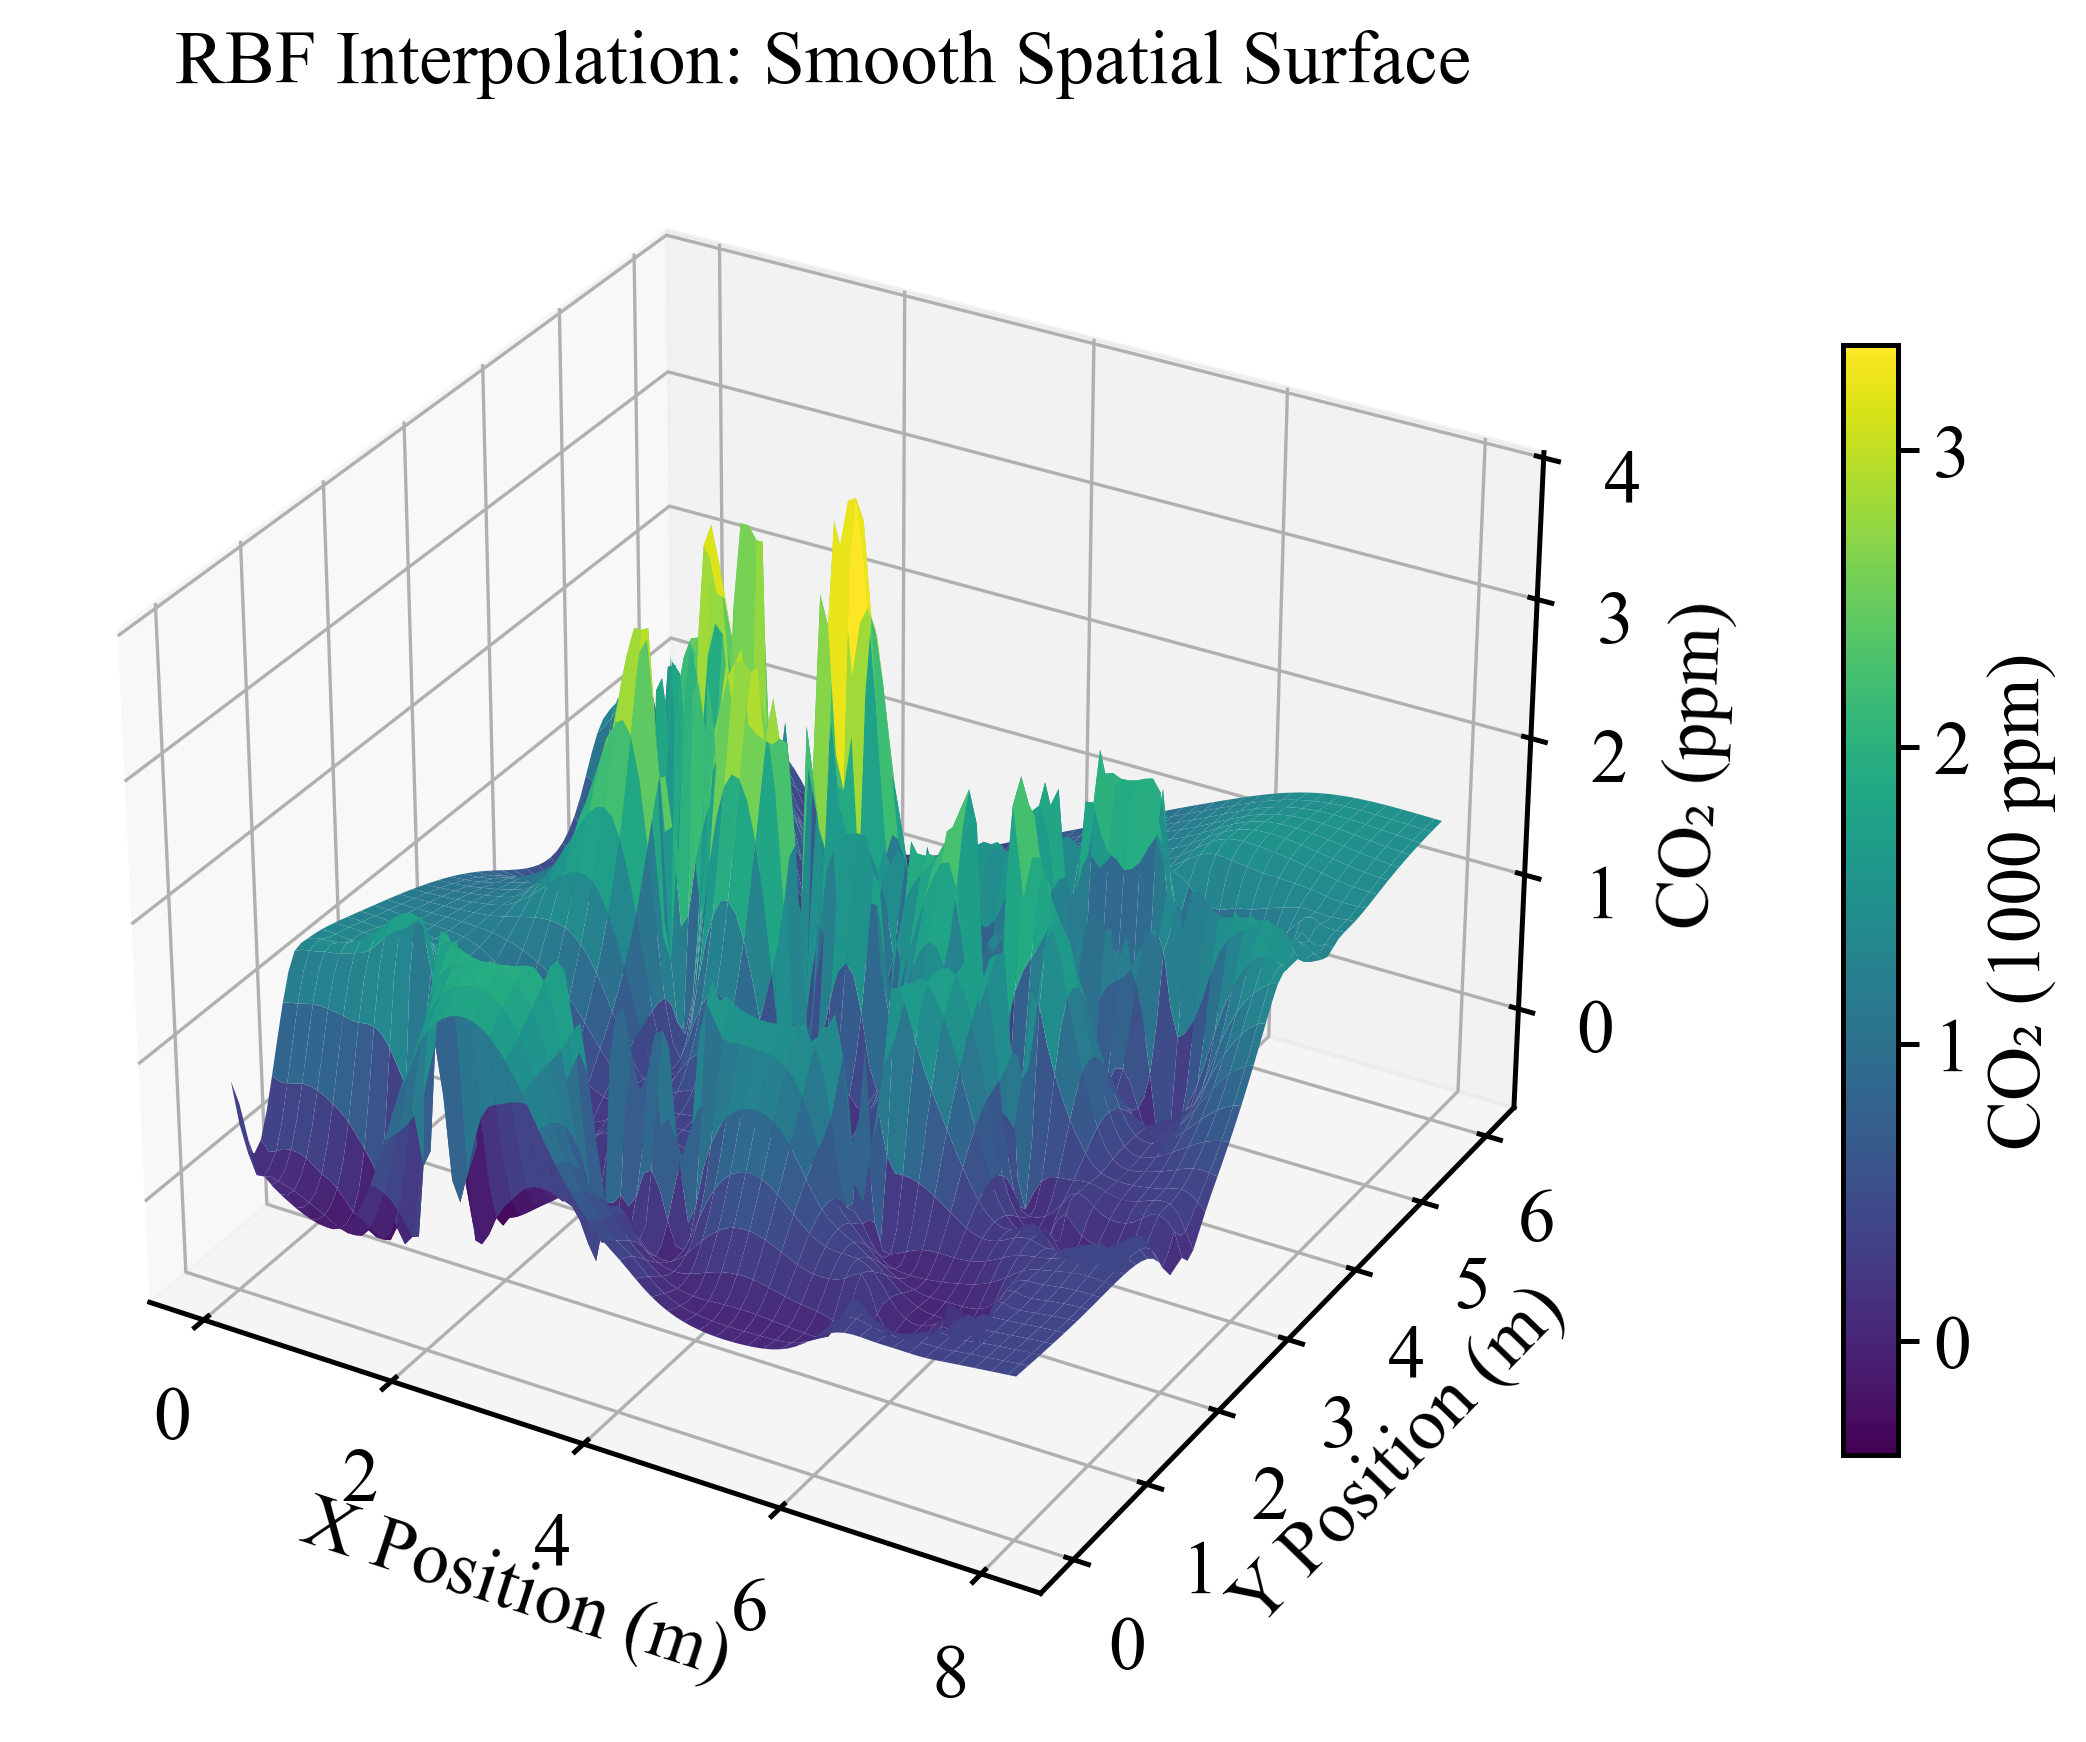
\includegraphics[width=0.6\textwidth]{Fig/04_rbf_surface.png} 
    \caption{Radial basis function interpolation of the diffused CO$_2$, the peaks show the possible leak points.}
    \label{fig:rbf}
\end{figure}

\subsection{Localizing the Leakage Sources}
To identify potential leak points from the interpolated CO$_2$ field, a peak detection algorithm is applied to locate local maxima in the concentration distribution. The algorithm scans the interpolated grid and identifies points that are higher than their immediate neighbors, indicating a local peak. To reduce false positives due to noise, a minimum prominence threshold is set, ensuring that only significant peaks are considered. The detected peaks are then ranked based on their concentration values, with the highest peaks being the most likely candidates for leak sources. The highest three peaks are averaged to estimate the most probable leak location, which is marked on the plot in Fig.~\ref{fig:peakmap}. This method provides a straightforward and computationally efficient approach to localizing leak points based on spatial concentration patterns, although further validation with ground truth data would be necessary for practical applications.
Figure~\ref{fig:peakmap} presents the detected local maxima (red crosses) in the RBF-interpolated CO$_2$ concentration field. The top three peaks (red stars) are selected as the most likely leakage candidates, and their averaged coordinates (cyan marker) estimate the final leak position. The estimated leak position lies close to the actual source location at $(3.0,\,3.5)$~m, demonstrating the effectiveness of the concentration-based spatial peak detection approach.
\begin{figure}
    \centering
    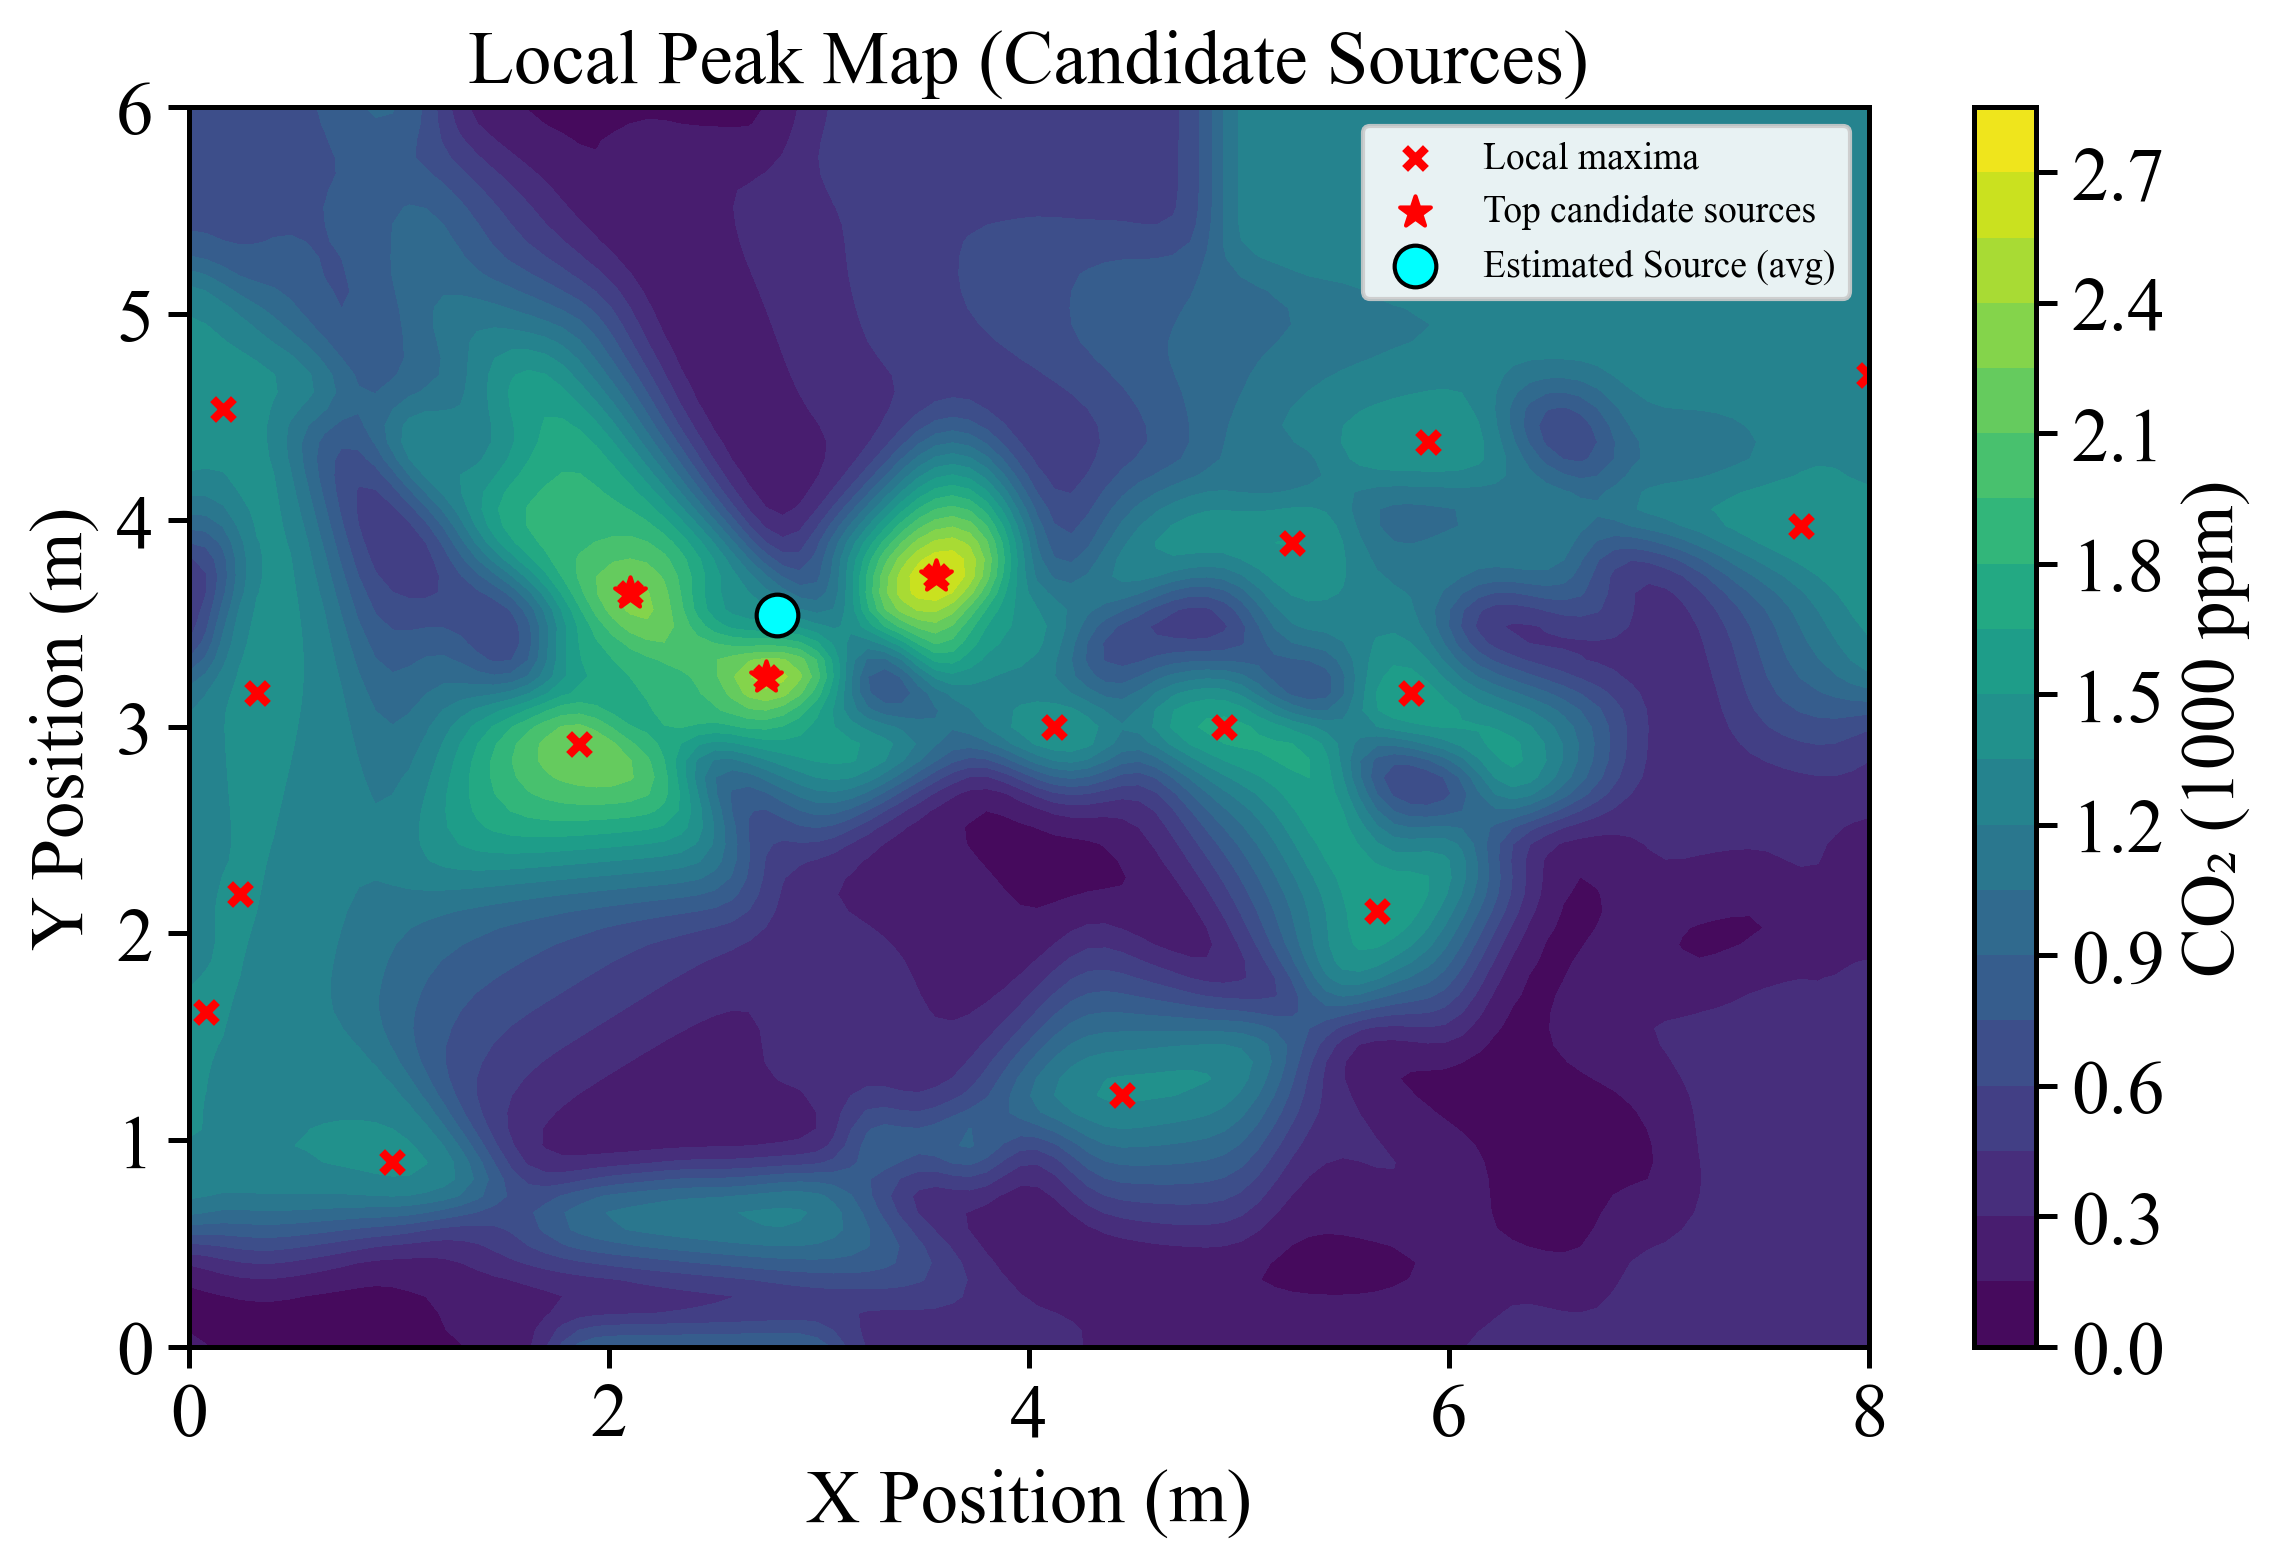
\includegraphics[width=0.6\textwidth]{Fig/09_peak_map.png} 
    \caption{Peak map showing the possible leak points in water tank, based on the local maxima points and averaging the highest three points.}
    \label{fig:peakmap}
\end{figure}

\subsection{Real Time Detection}
\begin{figure*}
    \centering
    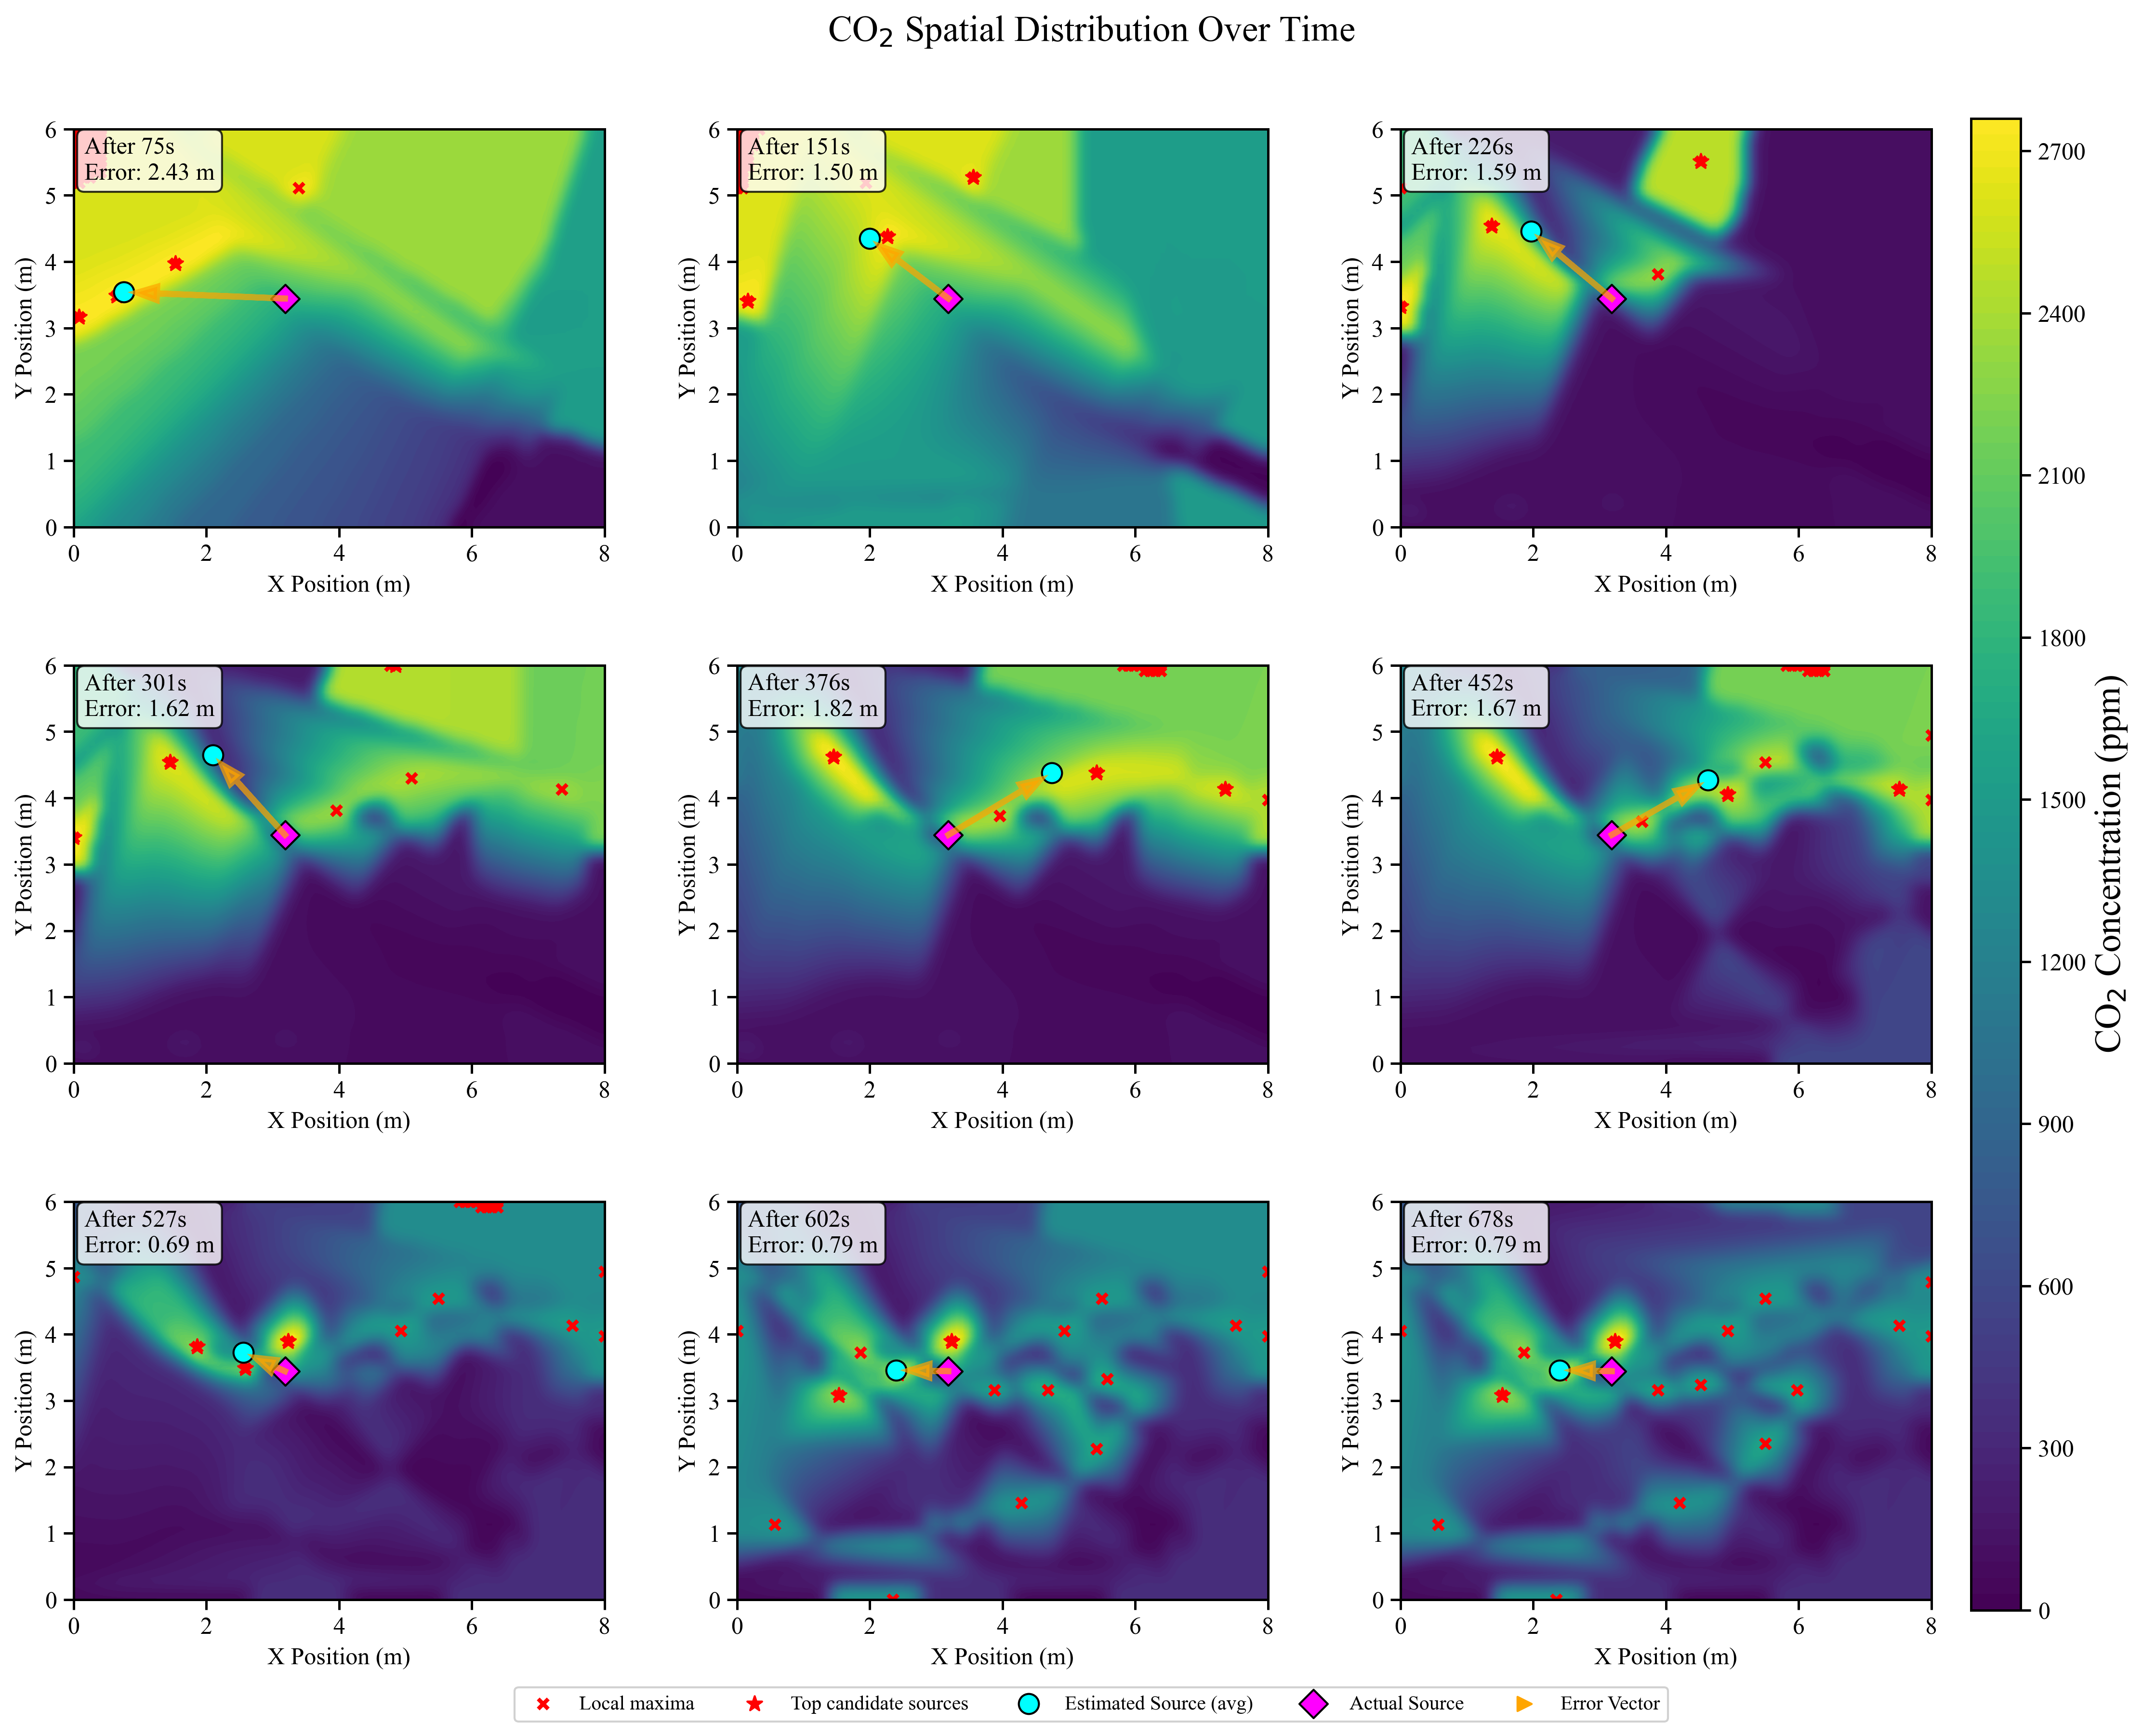
\includegraphics[width=0.95\textwidth]{Fig/co2_spatial_timewindows.png}
    \caption{CO$_2$ spatial distribution over time showing progressive improvement in leak localization. Each subplot represents a cumulative data window of 75 seconds, with the estimated source (cyan circle) converging toward the actual source (pink diamond) as localization error decreases from 2.43~m to 0.69~m.}
    \label{fig:windowed-time}
\end{figure*} 

\begin{figure}
    \centering
    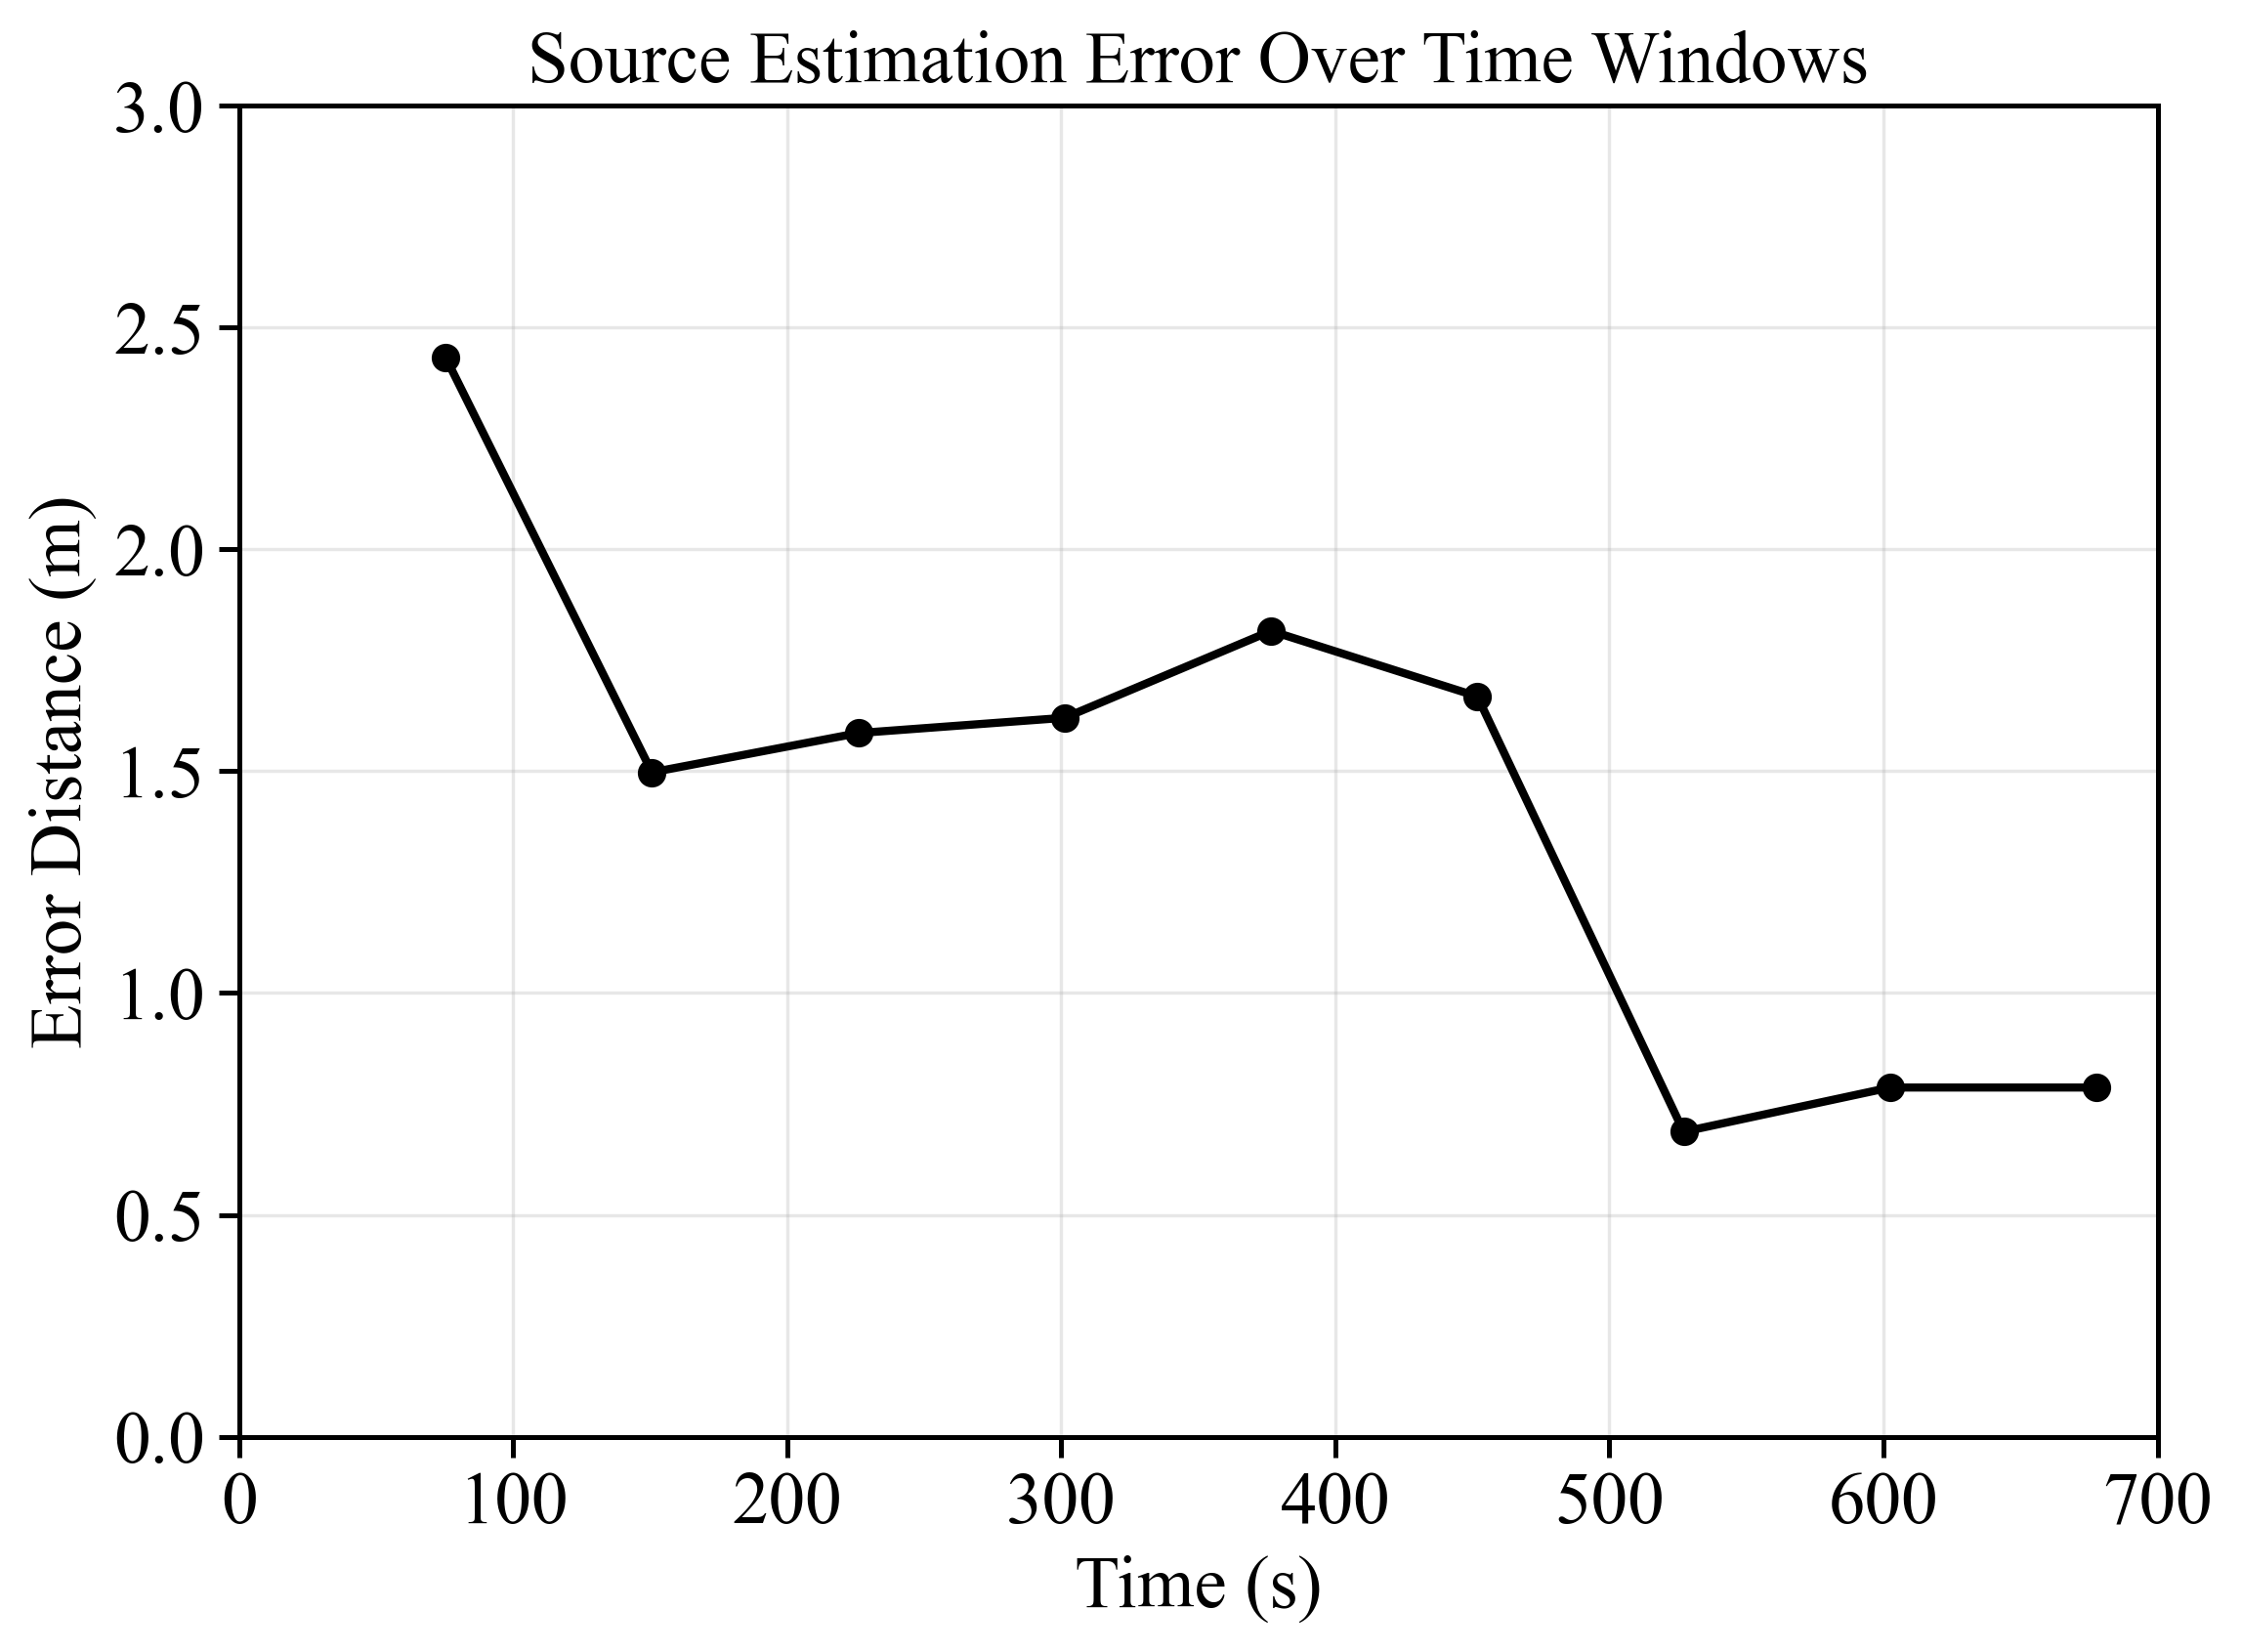
\includegraphics[width=0.48\textwidth]{Fig/source_estimation_error_over_time.png}
    \caption{Leak localization error over time, showing a decreasing trend as more data is collected.}
    \label{fig:error_over_time}
\end{figure}

As described in the previous sections, the robotic fish is maneuvering arbitrarily in the suspected area of the $\rm{CO_2}$ leakage, and collecting the data of diffused $\rm{CO_2}$ levels in water, with geo-tag and timestamps of the data, a feasibility is performed to see how accurately and effieciently, the same data can be used in real time for the robot to reach to the leak point. Considering the computational time limitation, the robot can process data after specified time. And each now data analysis provides the robots a better and better estimation of the leak source. For this purpose, the data is divided into multiple segments, each segment contains data collected over a period of 75 seconds. Each segment is processed using the same data analysis techniques as described in the previous sections, and the estimated leak point is recorded after each segment. 

Fig.~\ref{fig:windowed-time} shows a series of spatial CO$_2$ concentration maps generated at different time intervals, demonstrating the progressive refinement of leak localization as more data is collected. The figure displays nine snapshots taken at 75s, 151s, 226s, 301s, 376s, 452s, 527s, 602s, and 678s, respectively. Each subplot presents the RBF-interpolated concentration field with color gradients indicating CO$_2$ levels in ppm, where yellow regions represent high concentrations and purple regions indicate low concentrations. The actual leak source is marked with a pink diamond at coordinates $(3.0,\,3.5)$~m, while the estimated source position from the algorithm is shown as a cyan circle. Local maxima detected in the concentration field are indicated by orange crosses, and the top three candidate peaks are marked with red stars.

The localization error, displayed in the upper left corner of each subplot, demonstrates significant improvement over time. Starting with an initial error of 2.43~m after 75~s of data collection, the error progressively decreases to 1.50~m at 151~s, and continues to reduce through subsequent time windows. By 527~s, the error reaches 0.69~m, showing convergence toward the true leak location. This temporal progression illustrates the effectiveness of the incremental data processing approach, where each additional 75-second segment contributes to a more accurate spatial representation of the CO$_2$ distribution. The concentration maps become increasingly refined and localized around the actual source, validating the feasibility of real-time leak detection using the proposed methodology. The results demonstrate that even with limited initial data, the robotic fish can provide useful estimates that improve continuously as it collects more measurements, enabling adaptive navigation strategies for efficient leak localization. Fig.~\ref{fig:error_over_time} illustrates the trend of leak localization error over time, showing a clear decrease as more data is collected. The plot indicates that the error reduces from an initial value of 2.43~m to 0.69~m after 527~s, highlighting the effectiveness of the data-driven approach in refining leak source estimates with increasing measurement duration.

\section{CONCLUSION}
A bio-inspired robotic fish, AquaNavigator, is designed and developed to monitor the underwater CO$_2$ pipelines for any potential leakages. The robotic fish is equipped with a CO$_2$ sensor that can detect the presence of CO$_2$ in the water, keep record of the data, and tag it to the next possible surface position. The robotic fish can be deployed in the underwater environment to monitor the CO$_2$ pipelines for any potential leakages and provide real-time data to the operators. An indoor water tank is used to demonstrate the conditions, with a camera on the top to mimic the localization mechanism. A CO$_2$ pipeline leakage is setup in the bottom and the experiments show that the robotic fish is capable of localizing the area of leakage on CO$_2$. The experimental results successfully demonstrate that the proposed technique can be used to localize the leakage source of CO$_2$ in underwater pipelines, without using a swarm or multiple sensing  nodes to collect a combination of the spatial and temporal data. The results show that the spatial data alone, when collected for a sufficiently long time, can be used to localize the leak point. The proposed technique is computationally efficient and can be used in real-time applications. Future work will focus on improving the accuracy of the leak localization by incorporating temporal data and using more advanced interpolation techniques.
\bibliographystyle{IEEEtranDOI}
\bibliography{bibliography}
% \vspace{-1.2cm}
% \begin{IEEEbiography}
% [{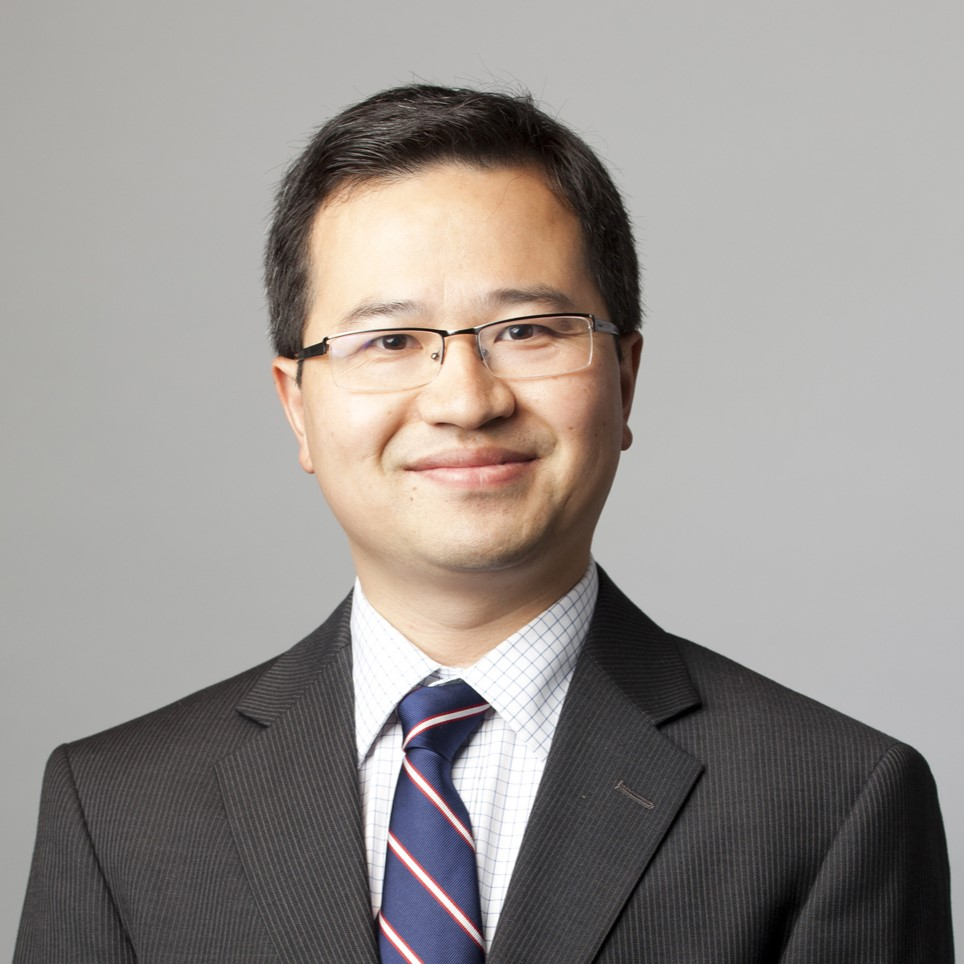
\includegraphics[width=1in,height=1in,clip,keepaspectratio]{Fig/Chen_Zheng_color.jpg}}]{Zheng Chen}
% is an Associate Professor Mechanical Engineering at the University of Houston (UH). He received B.E. degree in Electrical Engineering, M.E. degree in Control Science and Engineering from Zhejiang University, China in 1999 and 2002, and  Ph.D degree in Electrical Engineering from Michigan State University (MSU) in 2009. Dr. Chen joined the Department of Mechanical and Aerospace Engineering at the University of Virginia as a research associate in Sept. 2009. In July 20012, He joined Baker Hughes as a Research and Development engineer. From August 2013 to August 2017, Dr. Chen was an assistant professor in the Department of Electrical Engineering and Computer Science at Wichita State University. Dr. Chen is a senior member of IEEE. His research interests include electroactive polymers (EAPs), bio-inspired robotics, wearable devices, and renewable energy systems. Dr. Chen has received many prestigious awards, such as Kansas NSF EPSCoR First Award in Climate Change and Energy in 2015 and NSF CAREER Award in 2017. 
% \end{IEEEbiography}
% \vspace{-1.2cm}
% \begin{IEEEbiography}[{
\includegraphics[width=1in,height=1in,clip,keepaspectratio]{Fig/Umar_Masood.jpeg}}]{Muhammad Umar Masood} is currently a Ph.D. candidate in Mechanical Engineering at the University of Houston, where he specializes in bio-inspired robotics and underwater systems. With a background in Mechatronics Engineering from the National University of Sciences and Technology (NUST), his research focuses on the development of autonomous robotic fish for pipeline monitoring and $CO_2$ leakage detection. Umar has a passion for integrating advanced robotic technologies with practical environmental applications, aiming to enhance the operational efficiency and safety of underwater energy systems. His work has been recognized with several academic awards and he actively contributes to both IEEE conferences and journals in the fields of robotics.
% \end{IEEEbiography}
\end{document}